\documentclass{article}
\usepackage{authblk}
\usepackage{graphicx} % Required for inserting images


% Keywords command
\providecommand{\keywords}[1]
{
  \small	
  \textbf{\textit{Keywords---}} #1
}


\title{A new concept of the tensegrity based joint with an analysis}
\author[1]{Jan Zavřel}
\affil[1]{Czech Technical University in Prague, Faculty of Mechanical Engineering, Technická 4, Prague 6, 16000, Czech Republic}

\date{December 2023}


\begin{document}

\maketitle

\keywords{tensegrity, universal joint, revolute joint, stiffness}

\begin{abstract}
Tensegrity has recently been increasingly mentioned not only in architecture, but also in other fields such as biomechanics and robotics. Because of their properties, they are being used in new fields. In the field of biomechanics, their similarity to the structure of the human body is more than obvious. If we replace bones with rods or bodies and tendons with cables, the analogy is obvious. However, if we want to transfer tensegrity to robotics, then the standard joint design of a serial chiparallel robot cannot be taken directly from biomechanics or archtecture. The aim of this paper is to propose, analyze and experimentally verify a new revolute joint design applicable to serial robots. In the design and application, we can encounter some positive and negative properties of tensegrity structures, but also their limitations, especially the range of motion. The rotary tensegrity linkage can be easily extended to a universal joint and also be used to build a serial robot structure.
\end{abstract}

\section{Introduction}
Tensegrity (composed of tension and integrity, is a structural concept that involves a balance between tension and compression elements to create a stable  flexible structure  \cite{Ref_Snelson_1996} and \cite{Ref_Skelton_2001_introduction}. In a tensegrity structure, compression elements (usually rods or struts) do not directly touch each other but are instead connected by a network of continuous tension elements (usually cables).

Tensegrity structures have found applications in various fields, including architecture \cite{Ref_Skelton_2001_introduction}, engineering and robotics \cite{Ref_Krivosej_OWN_tensegrity_based_robots}, and biomechanics \cite{Ref_Scarr_BIO_elbow}, \cite{Ref_Xiongdun_BIO_wrist}, \cite{Ref_Jung_BIO_Flefural_Joint}, \cite{Ref_Li_BIO_Tensegritic_shoulder}, \cite{Ref_Sun_BIO_foot_tens_structure}, \cite{Ref_Lessard_BIO_lightweight_tens_joint} and \cite{Ref_Jung_BIO_Muscle_excitations_tens_joint}. Architects and designers appreciate their aesthetic appeal and the potential for creating innovative and efficient structures. Tensegrity principles are also employed in the development of flexible robotic systems and biomechanically inspired designs \cite{Ref_Xiongdun_BIO_wrist}, \cite{Ref_Jung_BIO_Muscle_excitations_tens_joint}.

The strengths and advantages are derived from the balance and interaction between tension and compression elements \cite{Ref_Skelton_2001_introduction} and can be summarized in the following properties.

\begin{itemize}
    \item{{\bf Redundancy and Load Distribution:} Tensegrity structures
            distribute loads efficiently throughout the system. The continuous tension network allows the structure to evenly distribute forces, minimizing localized stress points.}
    \item{{\bf Adaptive Response to External Forces:}
            Tensegrity structures are inherently flexible and can deform without losing stability. This adaptability enables them to absorb and redistribute forces, making them resilient to dynamic loads.}
    \item{{\bf High Strength-to-Weight Ratio:}
            Tensegrity structures often have a high strength-to-weight ratio, meaning they can carry significant loads relative to their mass. This efficiency is particularly advantageous in applications where weight is a critical factor, such as in lightweight constructions or structures meant for transportation.}
    \item{{\bf Tension Elements in Prestressed State:}
           Tension elements in a tensegrity structure are typically in a prestressed state, meaning they are under tension even in the absence of external loads. This prestressing contributes to the stability and immediate response to applied forces.}
    \item{{\bf Self-Tensioning Mechanism:}
           Tensegrity structures have a self-tensioning mechanism. When the structure experiences deformation or displacement, the tension elements automatically adjust to maintain equilibrium, ensuring continued stability.}
    \item{{\bf Resilience to Structural Failures:}
        Tensegrity structures can exhibit a certain degree of redundancy, meaning that even if a component fails, the overall structure can often remain standing. This resilience is valuable in applications where structural failure must be minimized or avoided.}
\end{itemize}

However, tensegrity structures also have their weaknesses \cite{Ref_Skelton_2001_introduction}, \cite{Ref_Hajzman_OWN_planning_method}, \cite{Ref_Krivosej_OWN_tensegrity_based_robots}. Understanding these limitations is crucial for designing and implementing tensegrity systems effectively. Here are some of the weaknesses associated with tensegrity structures. Tensegrity structures are highly sensitive to changes in tension and compression elements \cite{Ref_Krivosej_OWN_tensegrity_based_robots}. Precise engineering and construction are essential for maintaining stability \cite{Ref_Hajzman_OWN_planning_method} and \cite{Ref_Krivosej_OWN_tensegrity_based_robots}. Small errors in measurements or alterations in tension can significantly affect the overall performance. Designing tensegrity structures can be complex, requiring advanced mathematical modeling and analysis. Achieving the desired balance between tension and compression elements, as well as predicting the structure's behavior under different loads, can be challenging \cite{Ref_Krivosej_OWN_tensegrity_based_robots}. Tensegrity structures are known for their flexibility, which is advantageous in many applications. However, in some cases, this flexibility can be a limitation, especially in scenarios where rigidity is crucial.Tension elements, such as cables or tendons, are essential components of tensegrity structures. If a tension element fails or loses tension, it can lead to a collapse or deformation of the structure \cite{Ref_Skelton_2001_introduction}. Redundancy in tension elements can mitigate this risk but may not eliminate it entirely. While tensegrity structures have a high strength-to-weight ratio \cite{Ref_Krivosej_OWN_tensegrity_based_robots}, they may not be as well-suited for applications requiring extremely high load-bearing capacity. Certain configurations may have limitations in supporting heavy loads.

Although tensegrity structures have been used in various fields in recent years, their properties are often overestimated. Biomechanics and architecture are very important areas of application and foldable mechanisms generally as well.

There is an effort to replace common and experienced structures with tensegrities, but their use is not always appropriate. Due to their specific properties, they are predestined for light and rigid static constructions. For a purpose where movement is required, the use of tensegrity structures is no longer common. Although a typical example of tensegrity is the human body, where its elements are represented by tendons and bones, taking over the request is not usually suitable for other areas of application. A complex solution and redundancy then leads to a demanding solution to the task and its stability.

If we were to focus on the replacement of classical kinematic pairs (joints) with a tensegritic structure, then solving such a task is not easy. The solution of planar kinematic pairs lacks meaning in the reality, and such problems need to be solved comprehensively, like spatial problems. If we focus on the tasks of robotics, then in robotics there are mostly revolute joints, and that is due to its simplest structural nature. We can also encounter universal joint as well as spherical joint.

A large number of tensegrity structures are based on biomechanics and their movements are also limited. The limit angles of rotations $\varphi$ are thus very often in the range $\pm{\pi \over 2}$, often much less.

The aim of this work is to design a new type of the revolute joit and universal joit as well assuming a non-redundant number of cables..


\section{Revolute joint construction}
Unlike a common revolute joint or universal joint \cite{Ref_Dumas_STIFFNESS_stiffness_identification_6dof}, \cite{Ref_Jubien_STIFFNESS_Identicication_KUKA} and \cite{Ref_Dumas_STIFFNESS_identicication_serial_robots}, where the actuators are placed directly near the link, tensegrity structures are driven by cables. The cable drives are located outside the actual joint and are placed on other parts \cite{Ref_Li_BIO_Tensegritic_shoulder} of the structure or on the base frame \cite{Ref_Lessard_BIO_lightweight_tens_joint}.

For this reason, the design cannot be based on classical topology, but a completely new joint must be designed. One option is to wind the cable at the drive on a pulley \cite{Ref_Krivosej_OWN_tensegrity_based_robots}, and the other is to move the structure assuming a constant cable length. The idea and design of the actuator itself may be based on a planar problem, but the design will be a  spatial structure.



\subsection{Constant cable length drive design}
Consider a base of the planar tensegritic revolute joint formed by a body in the shape of T. The bottom part of the body (point O) is the revolute joint connected to the base frame and the top part is used to attach the cables (points U and V) (Fig.~\ref{fig:2D_revolute_constant_cable}).

\begin{figure}[!h]
    \centering
    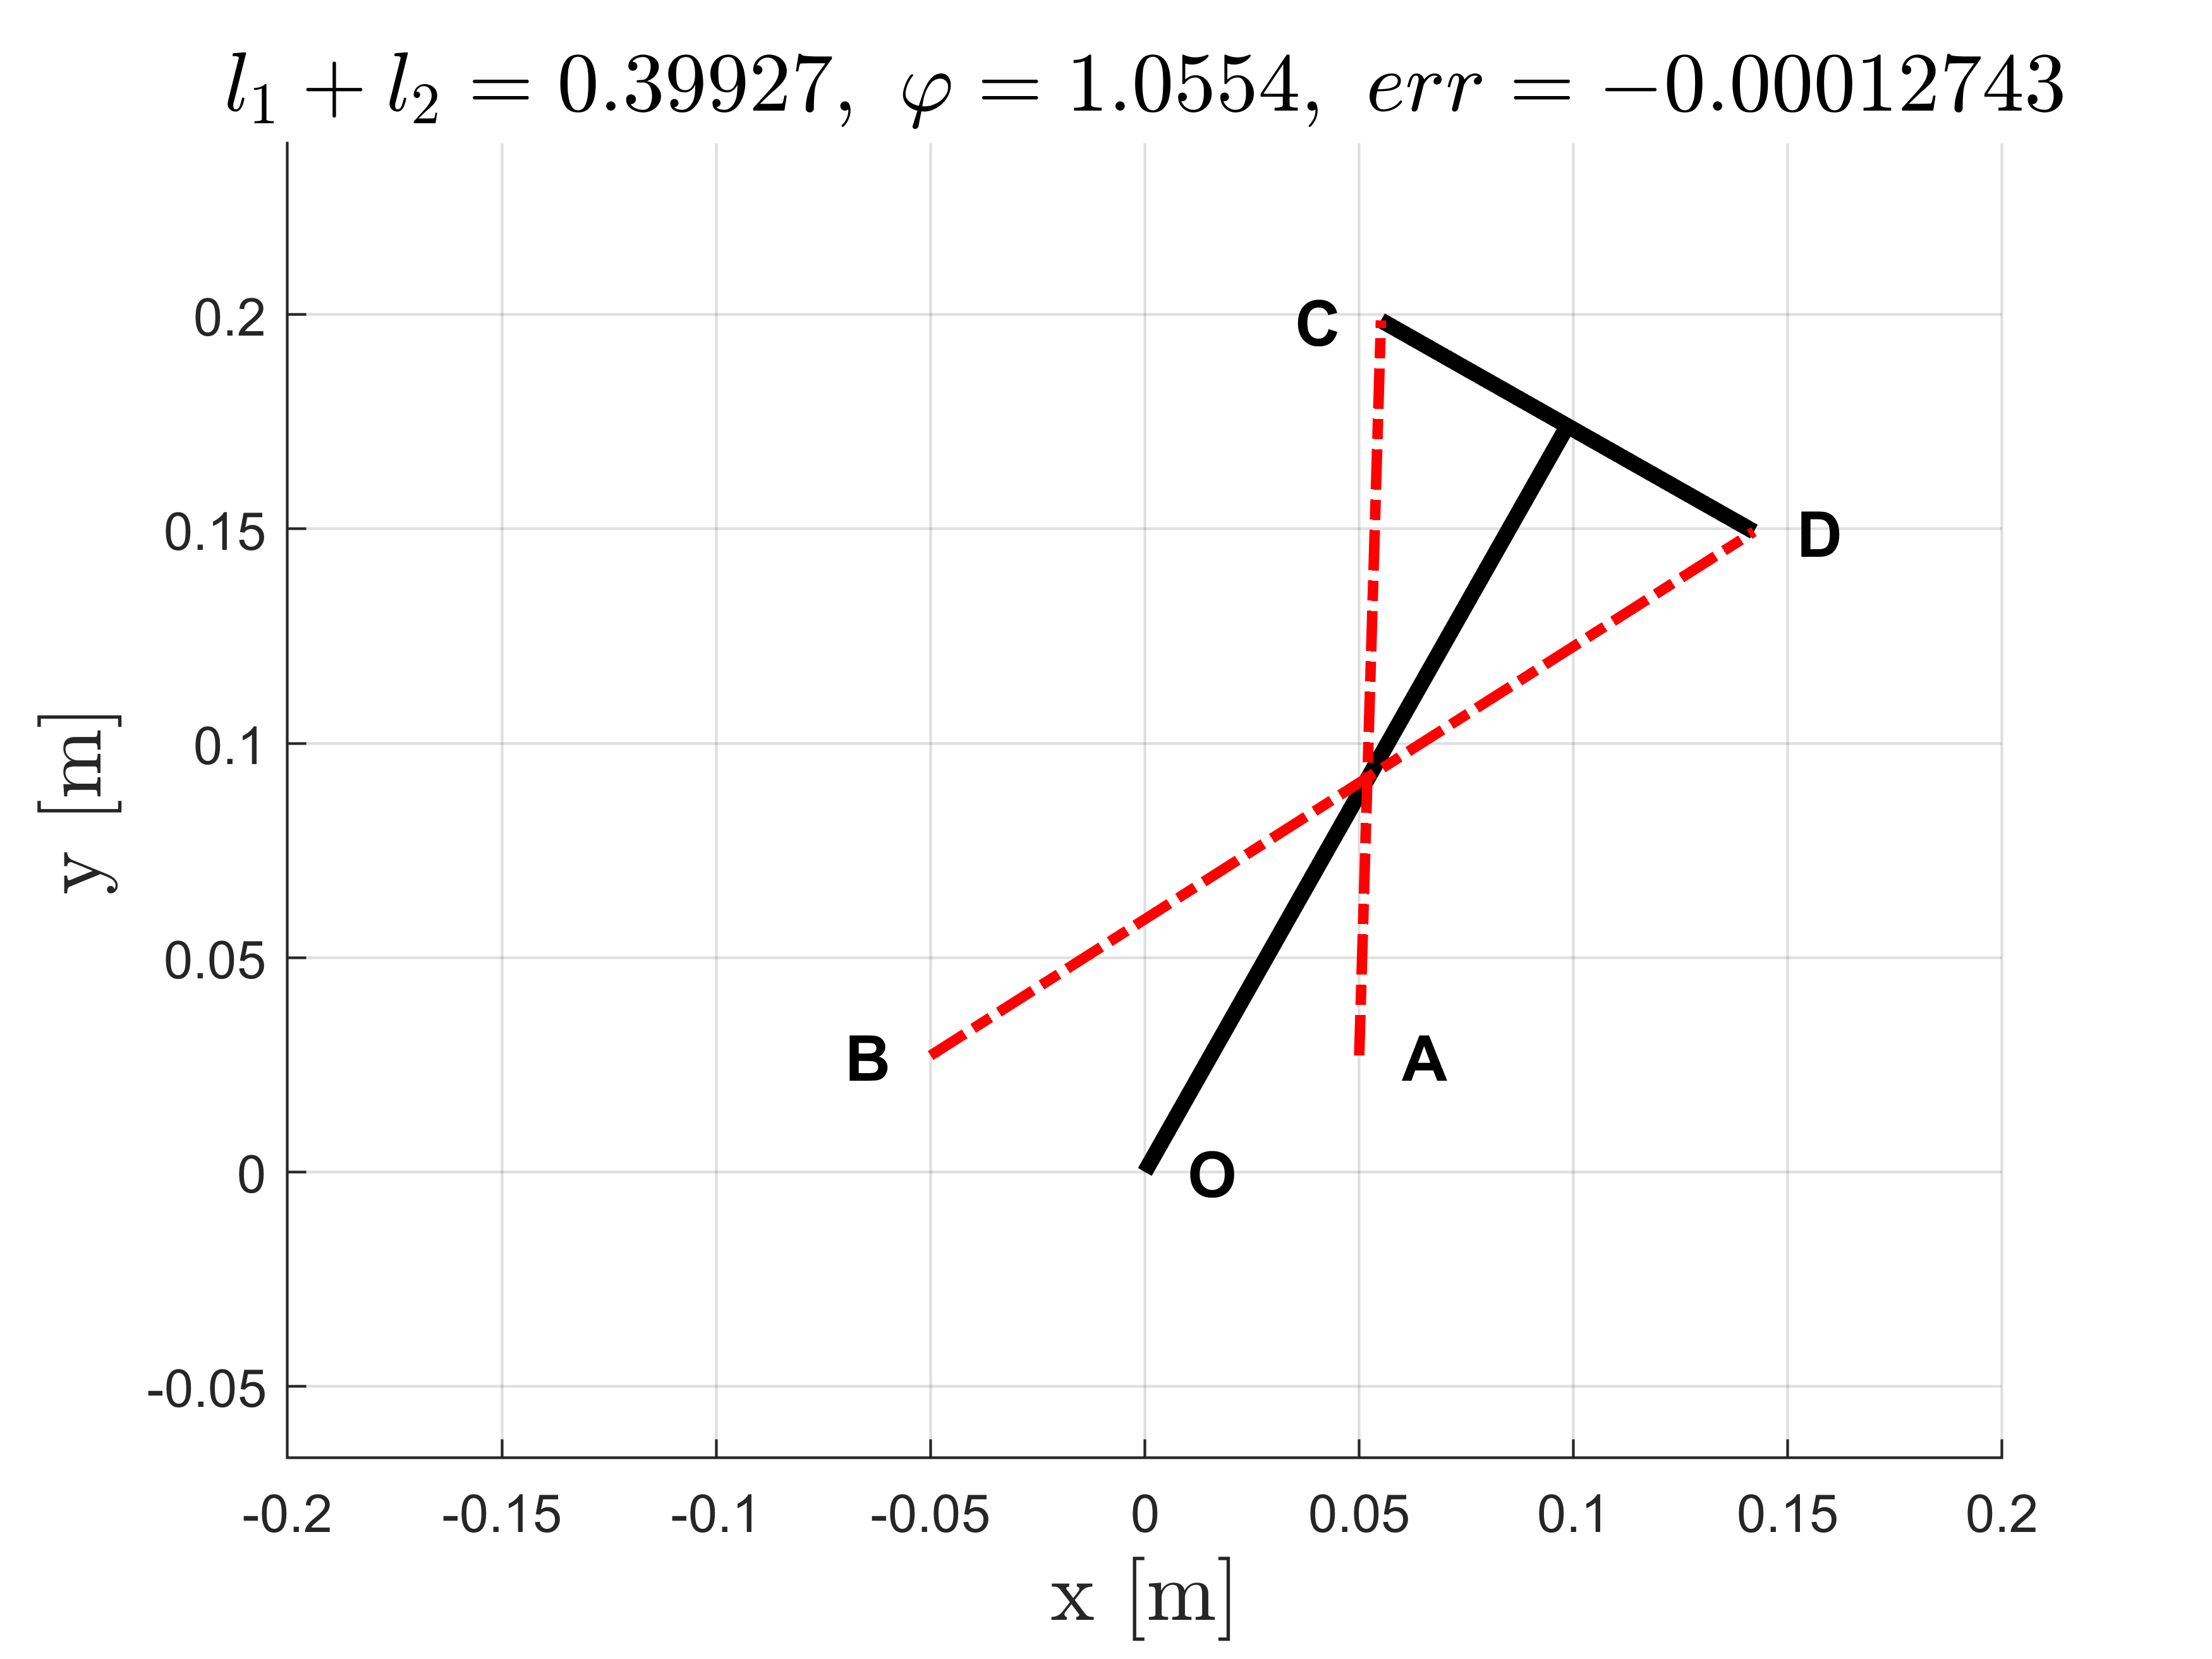
\includegraphics[width=8 cm]{figures/revolute_joint_scheme.png}
    \caption{Basic design of the 2D tensegritic revolute joint.}
    \label{fig:2D_revolute_constant_cable}
\end{figure}

The cable (red dash-dotted line) is attached at point A to the frame or other body and is guided through points U and V to the point B. Assuming a constant length of the cable, it is possible to place the cable drive on the upper part of the body.  By mutual shortening and lengthening of individual parts of the cable, the body will rotate around the artificial rotational point at point O.

The ideal position of points A and B for a constant length of cable during movement will certainly be at point O. However, this is not a suitable solution. Since the cables are supposed to be pre-tensioned in tensegritic structures, some imperfection in the constant length of the cable can be tolerated.  The cable can be pre-tensioned either by shortening its free length, or by placing pre-tensioning springs inside the cable (e.g. at points A and B).

For a tensegrity joint (Fig.~\ref{fig:2D_revolute_constant_cable}), the length of the cable will change only minimally when it rotates by $\pm{\pi \over 4}$ measured from the vertical axis about point O. The change in the length of the cable (the reference length is taken from the vertical position of the body) is shown in Fig~\ref{fig:cable_length_deviatiopn}.

\begin{figure}[h]
    \centering
    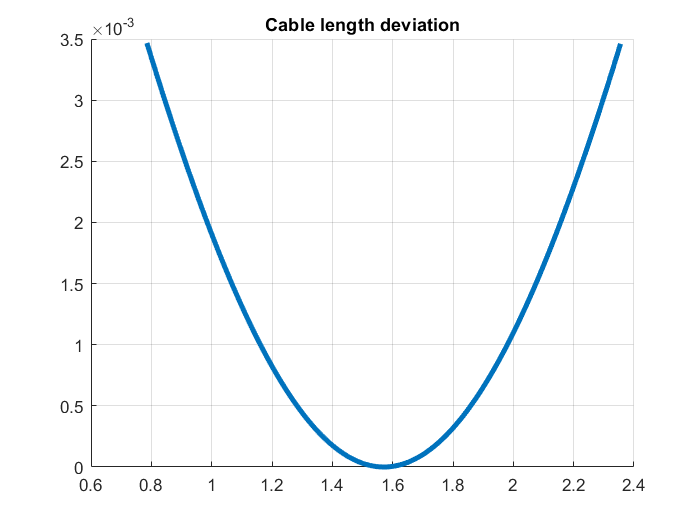
\includegraphics[width=8 cm]{figures/cable_length_deviation.png}
    \caption{Cable length deviation}
    \label{fig:cable_length_deviatiopn}
\end{figure}

\begin{figure}[h]
    \centering
    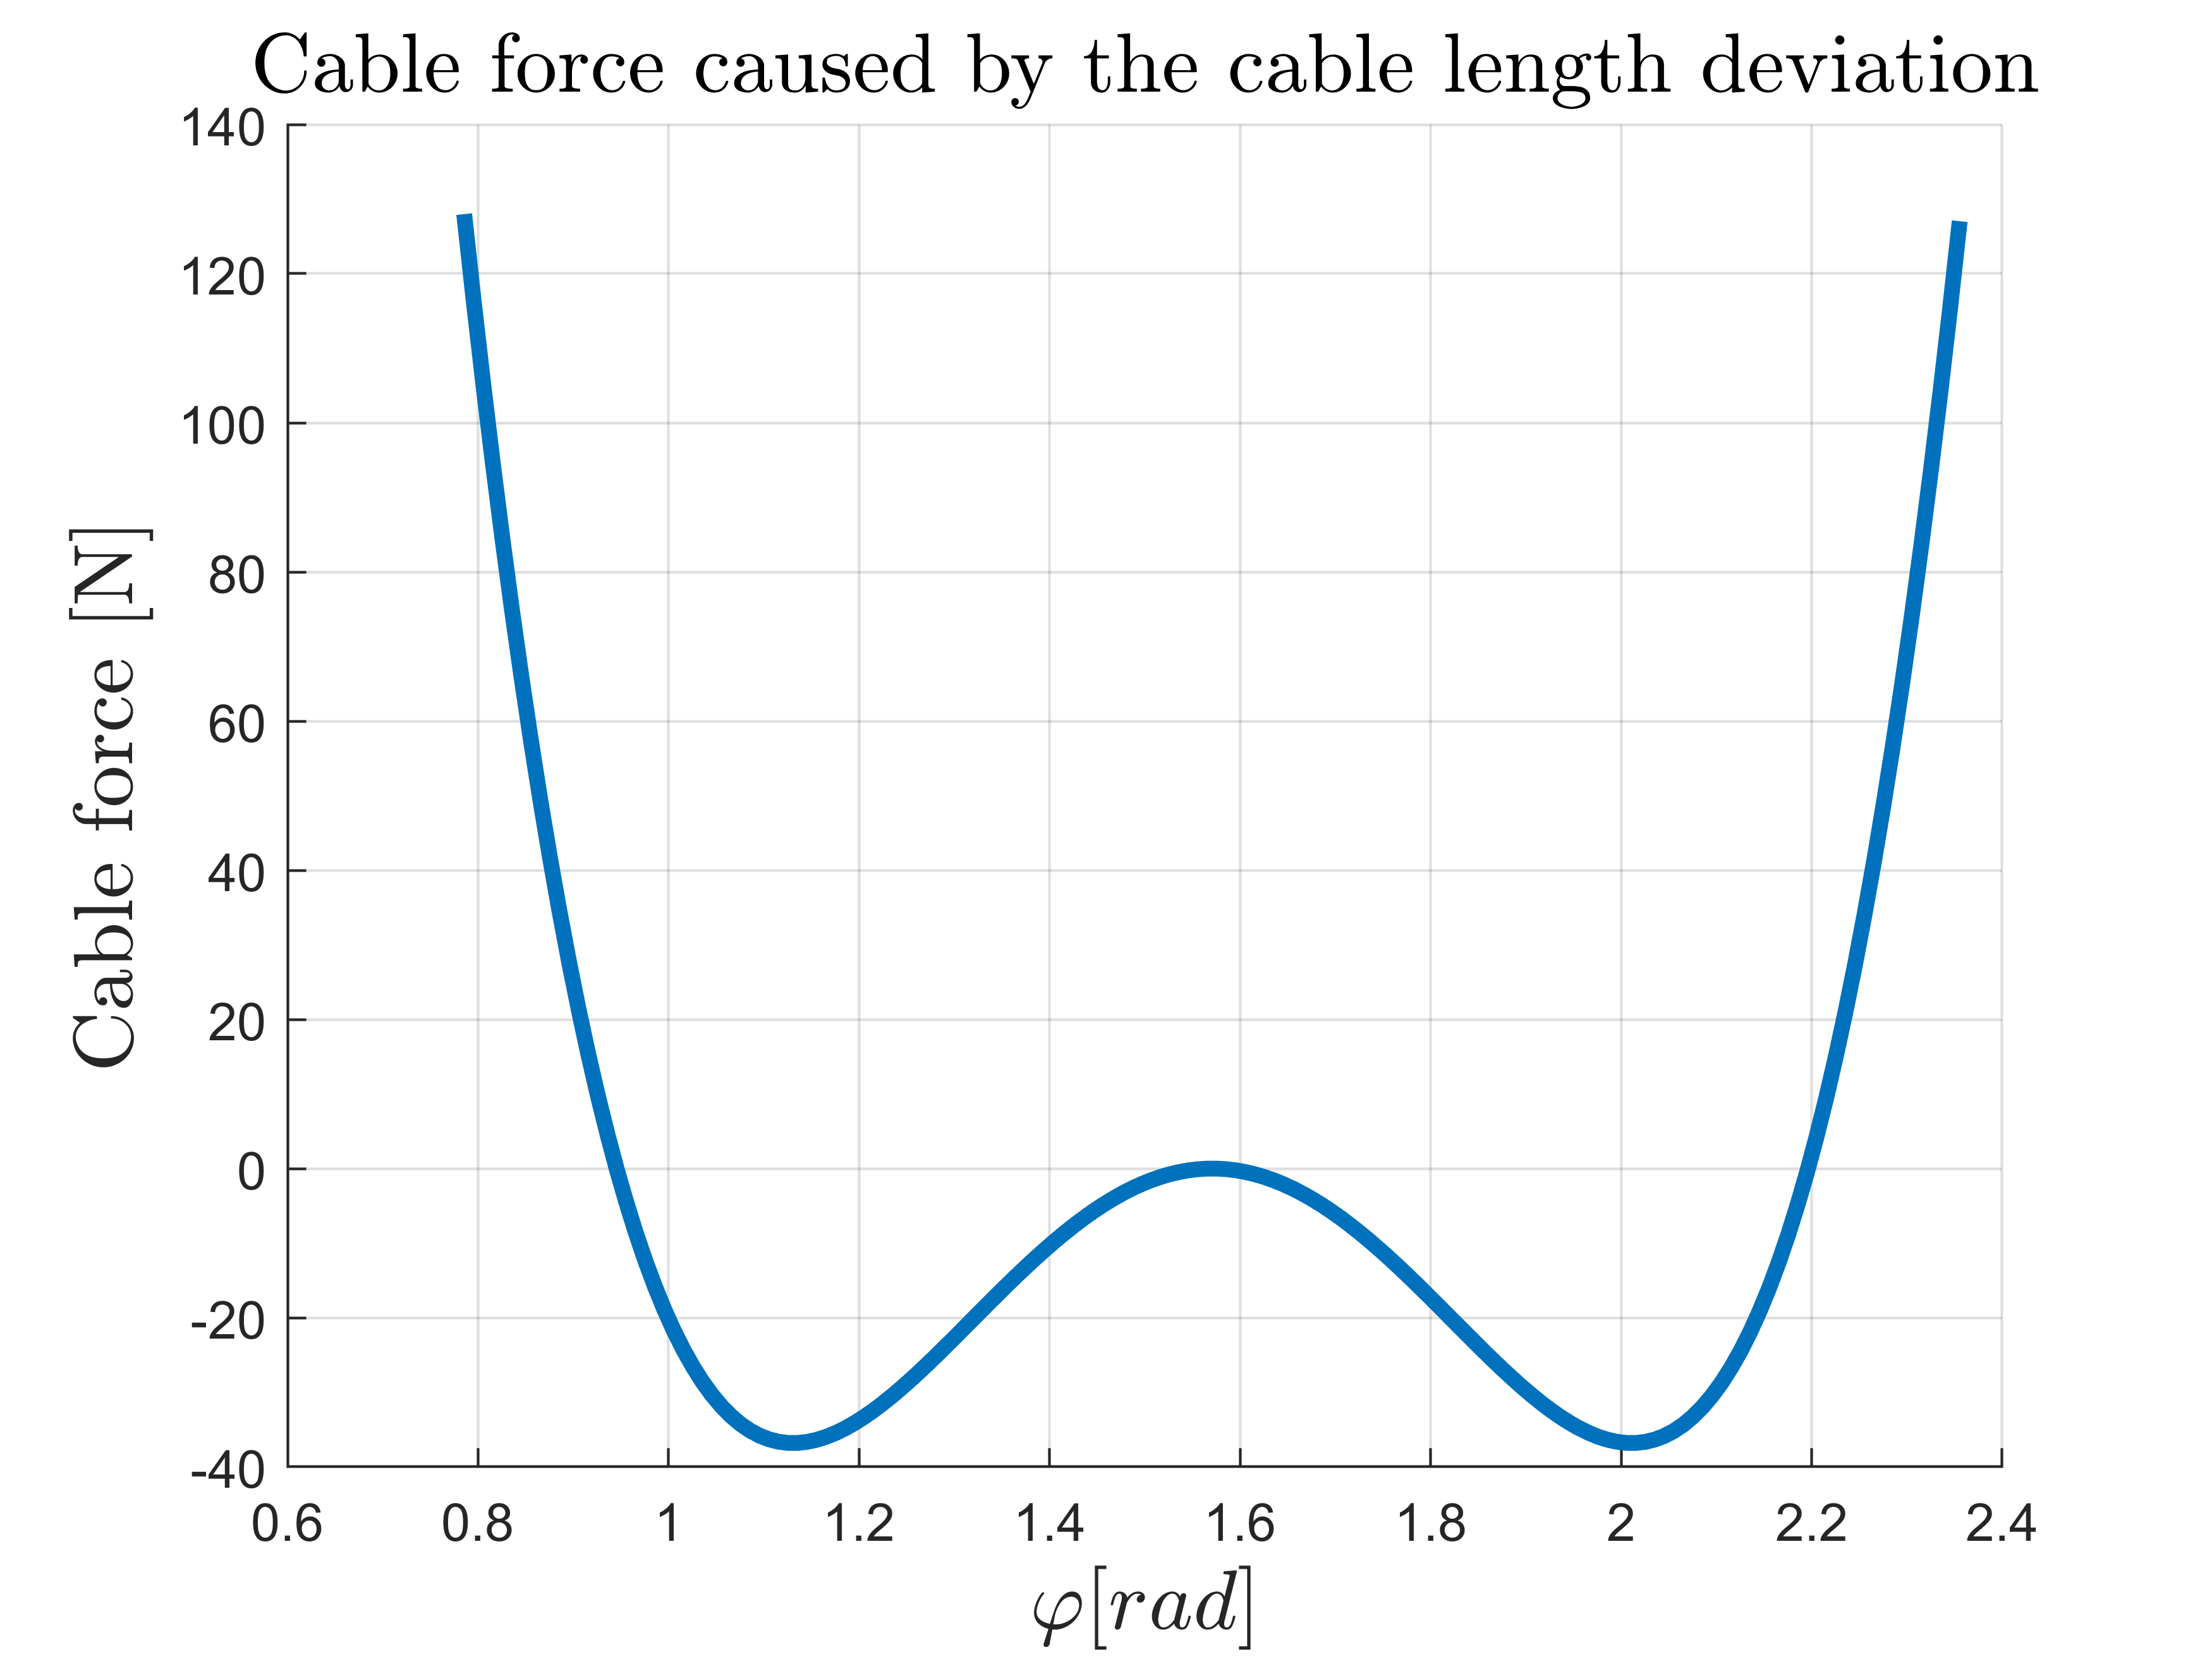
\includegraphics[width=8 cm]{figures/cable_force_deviation.png}
    \caption{Caption}
    \label{fig:cable_force_deviation}
\end{figure}

If we consider the stiffness $k=2.5e5\ Nm^{-1}$ of the cable for the structure, then the cable force will be as in the Fig.~\ref{fig:cable_force_deviation}.

For the pretension of the cable $F_p=200\ N$, such a movement is then completely sufficient to ensure the pretension in the cable.

\subsection{Spatial tensegritic revolute joint}

Based on the design of 2D tensegrity revolute joint, the concept of spatial tensegritic revolute joint was created. The concept is based on two oppositely oriented and $\pi \over 2$ twisted bodies (body 2 and body 3) . Their interconnection, which creates a revolute/universal joint, is created by four cables of constant lengths (cables $c_3,\ c_4,\ c_5\ c_6$). The movement is provided by two cables, in the case of revolute joint (cables $c_1,\ c_2$ or $c_7,\ c_8$). The universal joint is composed of two revolute joints, it is drived by four cables (cables $c_1,\ c_2,\ c_7,\ c_8$). In analogy with the design of the planar rotary tensegrity joint Fig.~\ref{fig:2D_revolute_constant_cable}, the drive is always performed by a single cable guided from the point $A_2$ to the point $B_2$ over points $U_2$ and $V_2$. There is placed a pulley with drive between points $U_2$ and $V_2$. Analogically there is a second movement by a cable guided from the point $A_3$ to the point $B_3$ over points $U_3$ and $V_3$. There is placed a second pulley with a drive between points $U_3$ and $V_3$.

\begin{figure}[h!]
    \centering
    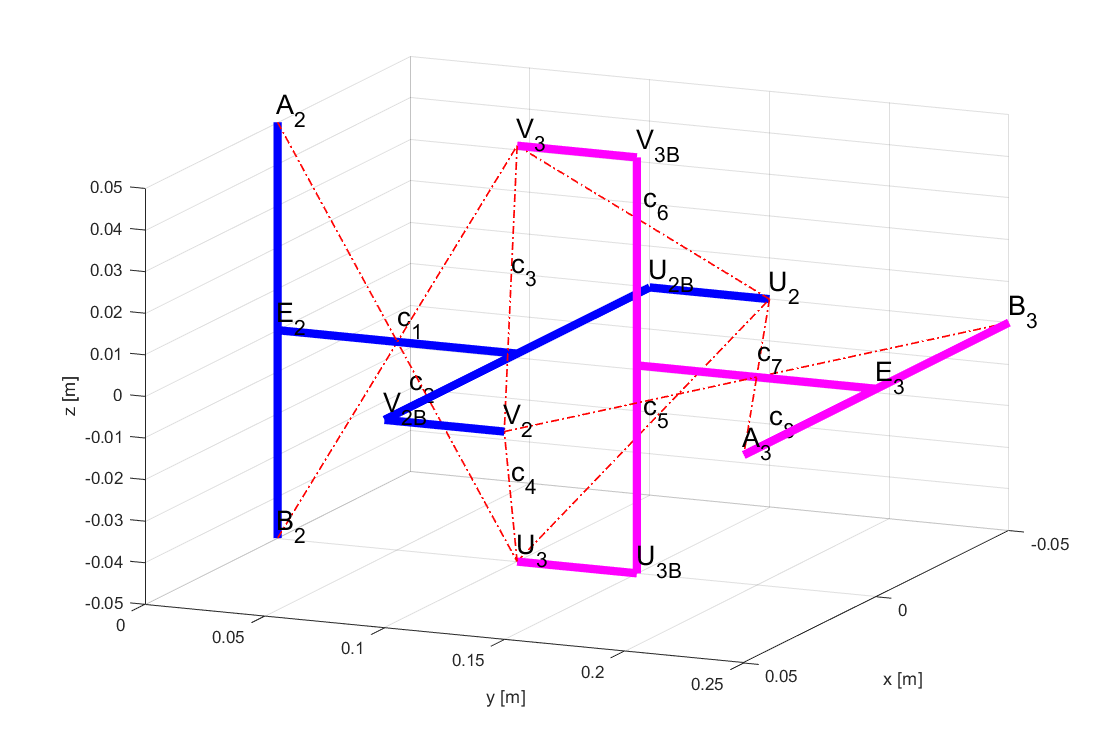
\includegraphics[width=12cm]{figures/universal_joint.png}
    \caption{A scheme of the revolute and the universal joint. Body 2 - blue, body 3 - magenta.}
    \label{fig:revolute_universal_joint}
\end{figure}

The motion of the end-point $E_3$ can be described in the matrix form for the universal joint (Fig.~\ref{fig:universal_joint_scheme}).

Position $r_{1_{E_3}}$ of the end-point $E_3$ can be described in the world-frame coordinate system 1 ($x_1,\ y_1,\ z_1$) like

\begin{equation}
    r_{1{E_3}} = T_{13} r_{3{E_3}},
\end{equation}

where $T_{13}$ is the transform matrix from the coordinate system 3 to the coordinate system 1 and $r_{3{E_3}}$ is the position vector ef the point $E_3$ in the coordinate system 3.

The transform matrix $T_{13}$ is composed from two rotation matrices (rotations $\varphi_x$ and $\varphi_z$) and two movements in the $y$ axis.

The transform matrices for rotations are 

\begin{equation}
    T_{\varphi_x}({\varphi_x})=
    \left[
    \begin{array}{cccc}
        1  &0         &0        &0\\
        0  &\cos(\varphi_x)  &-\sin(\varphi_x) &0\\
        0  &\sin(\varphi_x)  &\cos(\varphi_x) &0\\
        0  &0         &0        &1\\
    \end{array}
    \right]
\end{equation}

\begin{equation}
    T_{\varphi_z}({\varphi_z})=
    \left[
    \begin{array}{cccc}
        \cos(\varphi_z)   &-\sin(\varphi_z)    &0  &0\\
        \sin(\varphi_z)   &\cos(\varphi_z)    &0  &0\\
        0          &0           &1  &0\\
        0          &0           &0  &1\\
    \end{array}
    \right]
\end{equation}

and for the translation in the $y$ axis is

\begin{equation}
    T_{y}(y)=
    \left[
    \begin{array}{cccc}
        1   &0    &0  &0\\
        0   &1    &0  &y\\
        0   &0    &1  &0\\
        0   &0    &0  &1\\
    \end{array}
    \right]
\end{equation}

The resulting transformation $T_{13}$ is therefore

\begin{equation}
    T_{13} = T_{y}(h_1) T_{\varphi_x}(\varphi_x) T_{\varphi_y}(\varphi_x) T_{y}(l_3)
\end{equation}

The position vector $r_3{E_3}$ of the point $E_3$ in the coordinate system 3 is then

\begin{equation}
    r_3{E_3}=
    \left[
    \begin{array}{c}
        0\\
        0\\
        0\\
        1\\
    \end{array}
    \right]
\end{equation}

The dimension $h_1$ is the distance between points $E_2$ and $O_2$, and $l_3$ is the distance between points $O_3$ and $E_3$, where $h_1 = 0.125\ m$. Points $O_2$ and $O_3$, where $l_3 = 0.125\ m$ are in the middle of the universal joint or revolute joint. These points are located in the identical place and are in the artificial middle of the tensegrity joint (Fig.~\ref{fig:revolute_universal_joint}).

The position of the end-point $E_3$ is also given by equations

\begin{eqnarray}
   x_{1M} &=& -l_3\cos(\varphi_x)\sin(\varphi_z)\\
   y_{1M} &=& h_1 + l_3 \cos(\varphi_x) \cos(\varphi_z)\\
   z_{1M} &=& l_3 \sin(\varphi_x)\\
\end{eqnarray}


\begin{figure}[h!]
    \centering
    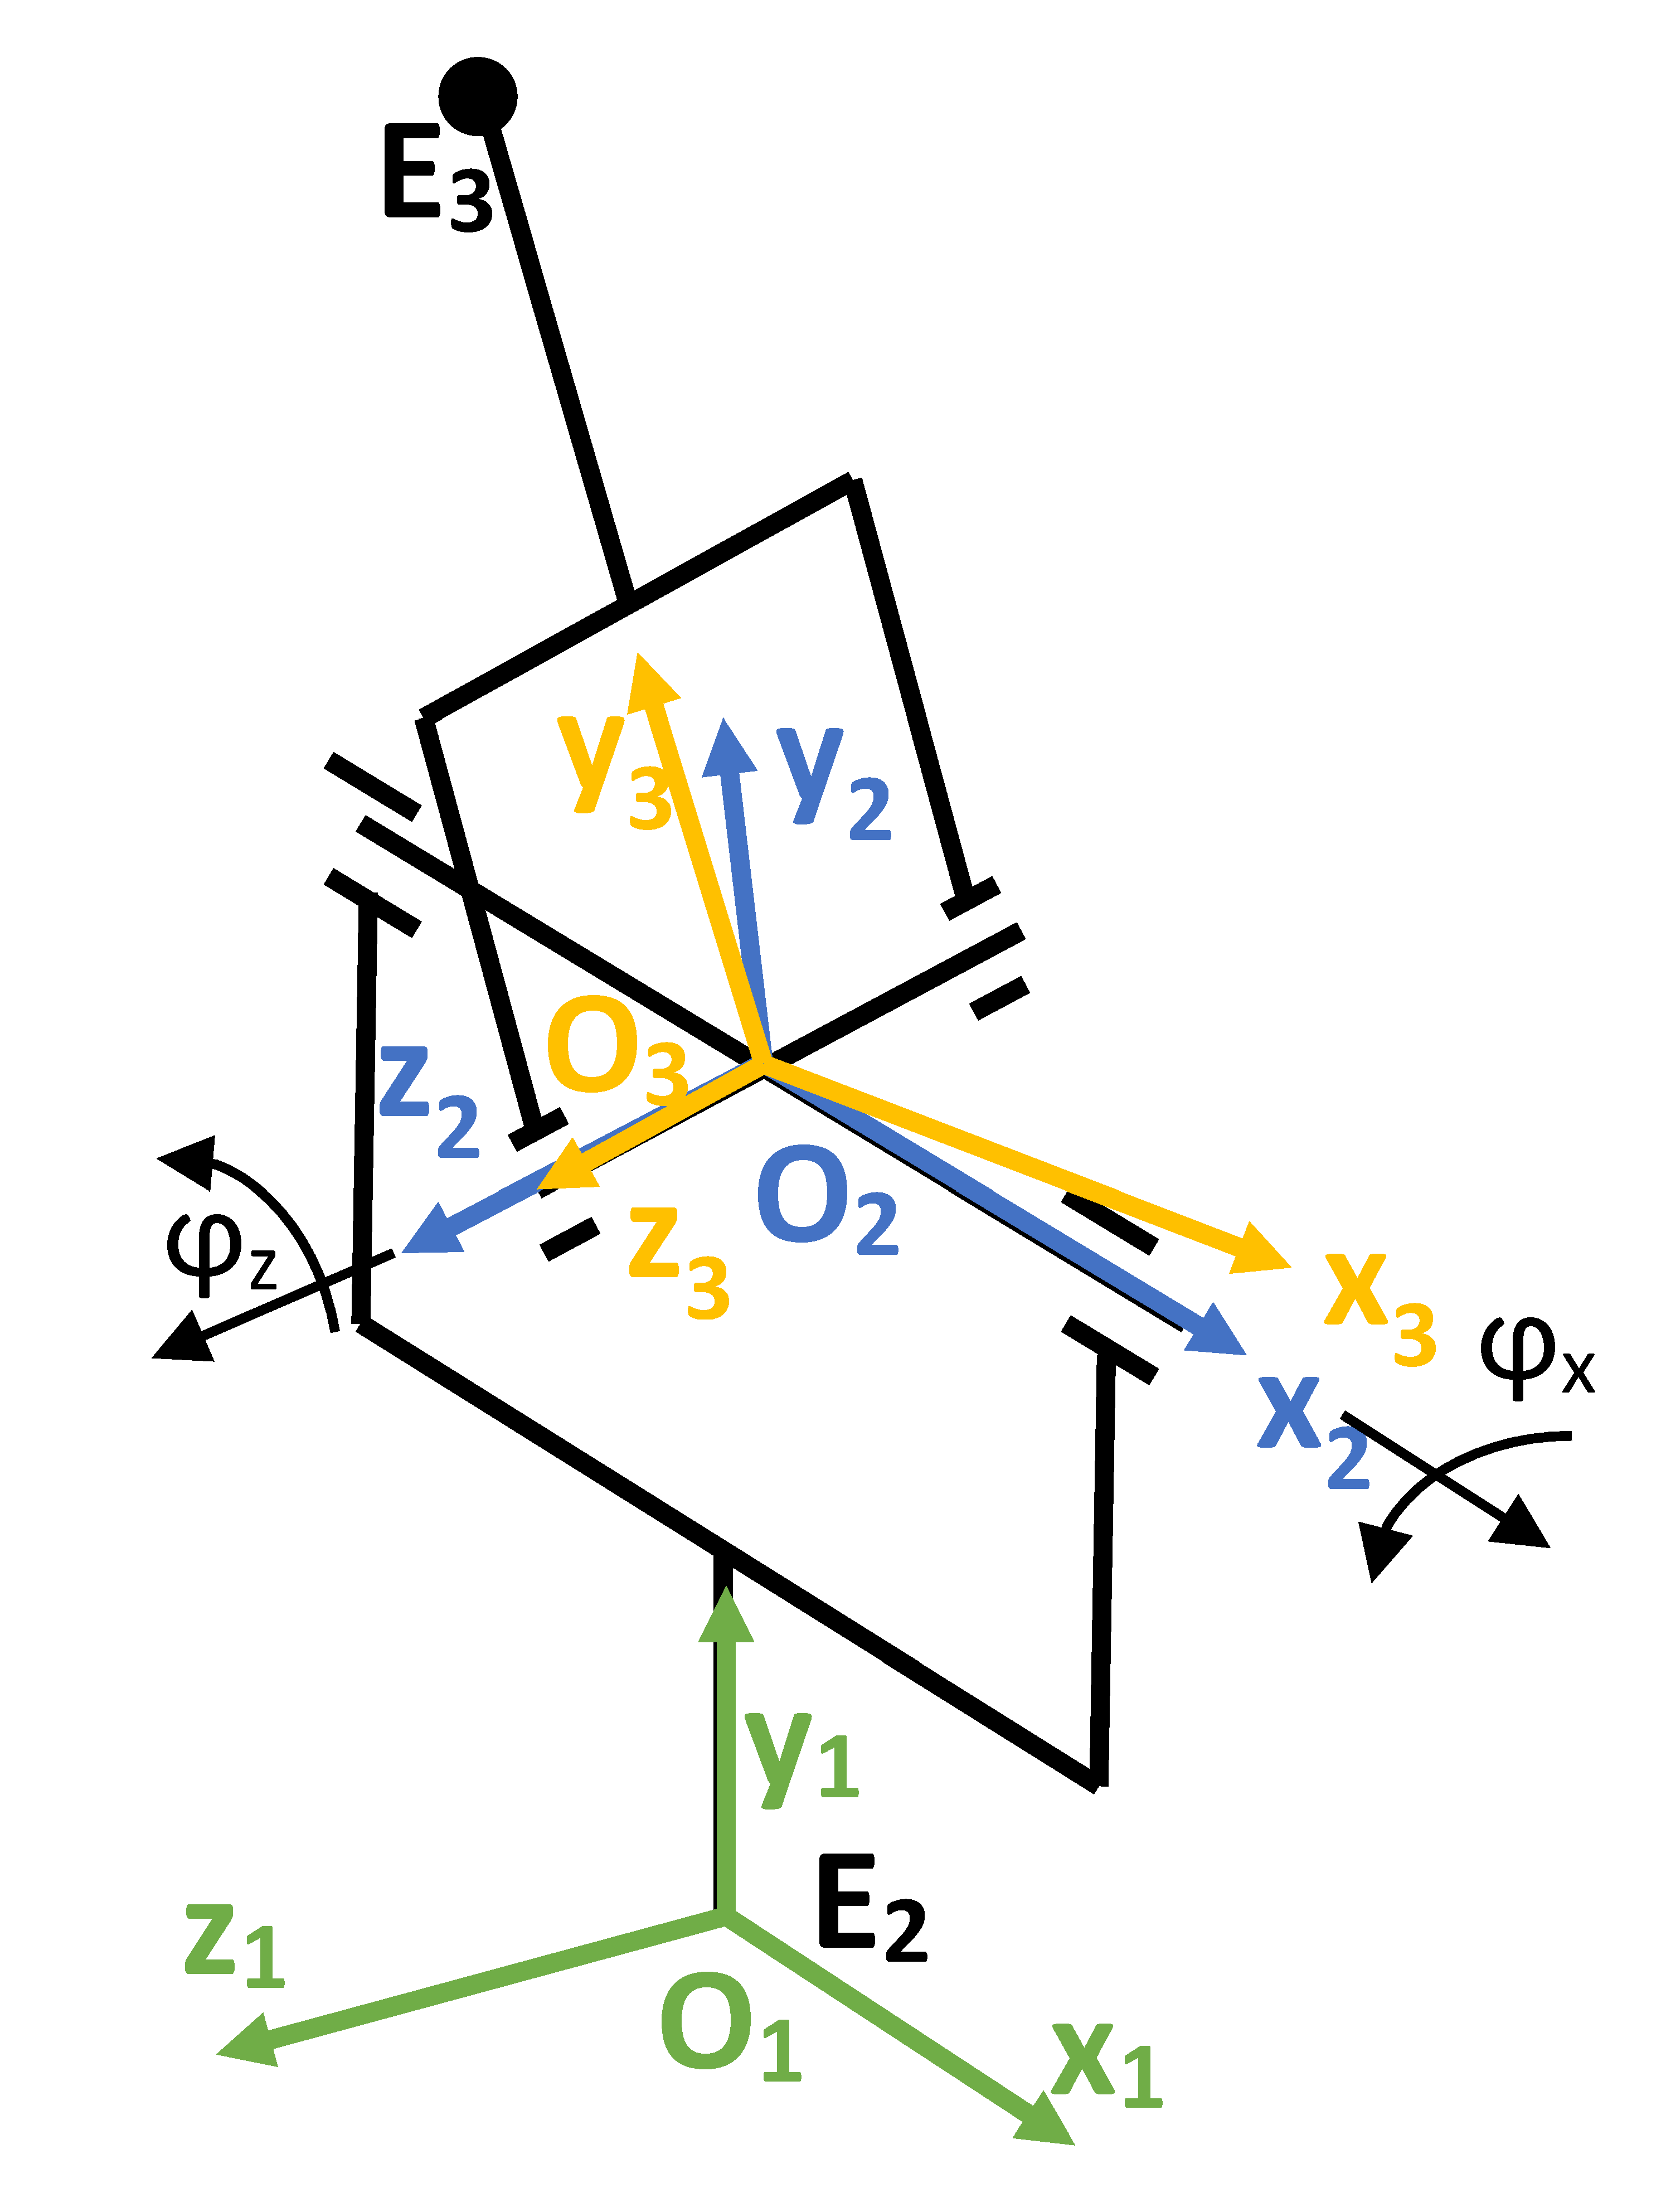
\includegraphics[width=5cm]{figures/universal_joint_scheme.png}
    \caption{Kinematic scheme of the universal joint.}
    \label{fig:universal_joint_scheme}
\end{figure}

Depending on the choice of coordinates (direct or inverse kinematics) for the range of $\varphi_x \in <-{\pi \over 3},\ {\pi \over 3}>$ and $\varphi_z \in <-{\pi \over 3},\ {\pi \over 3}>$ angles, the map of the working space of point $E_3$ is shown in the figures 

\begin{figure}[h!]
    \centering
    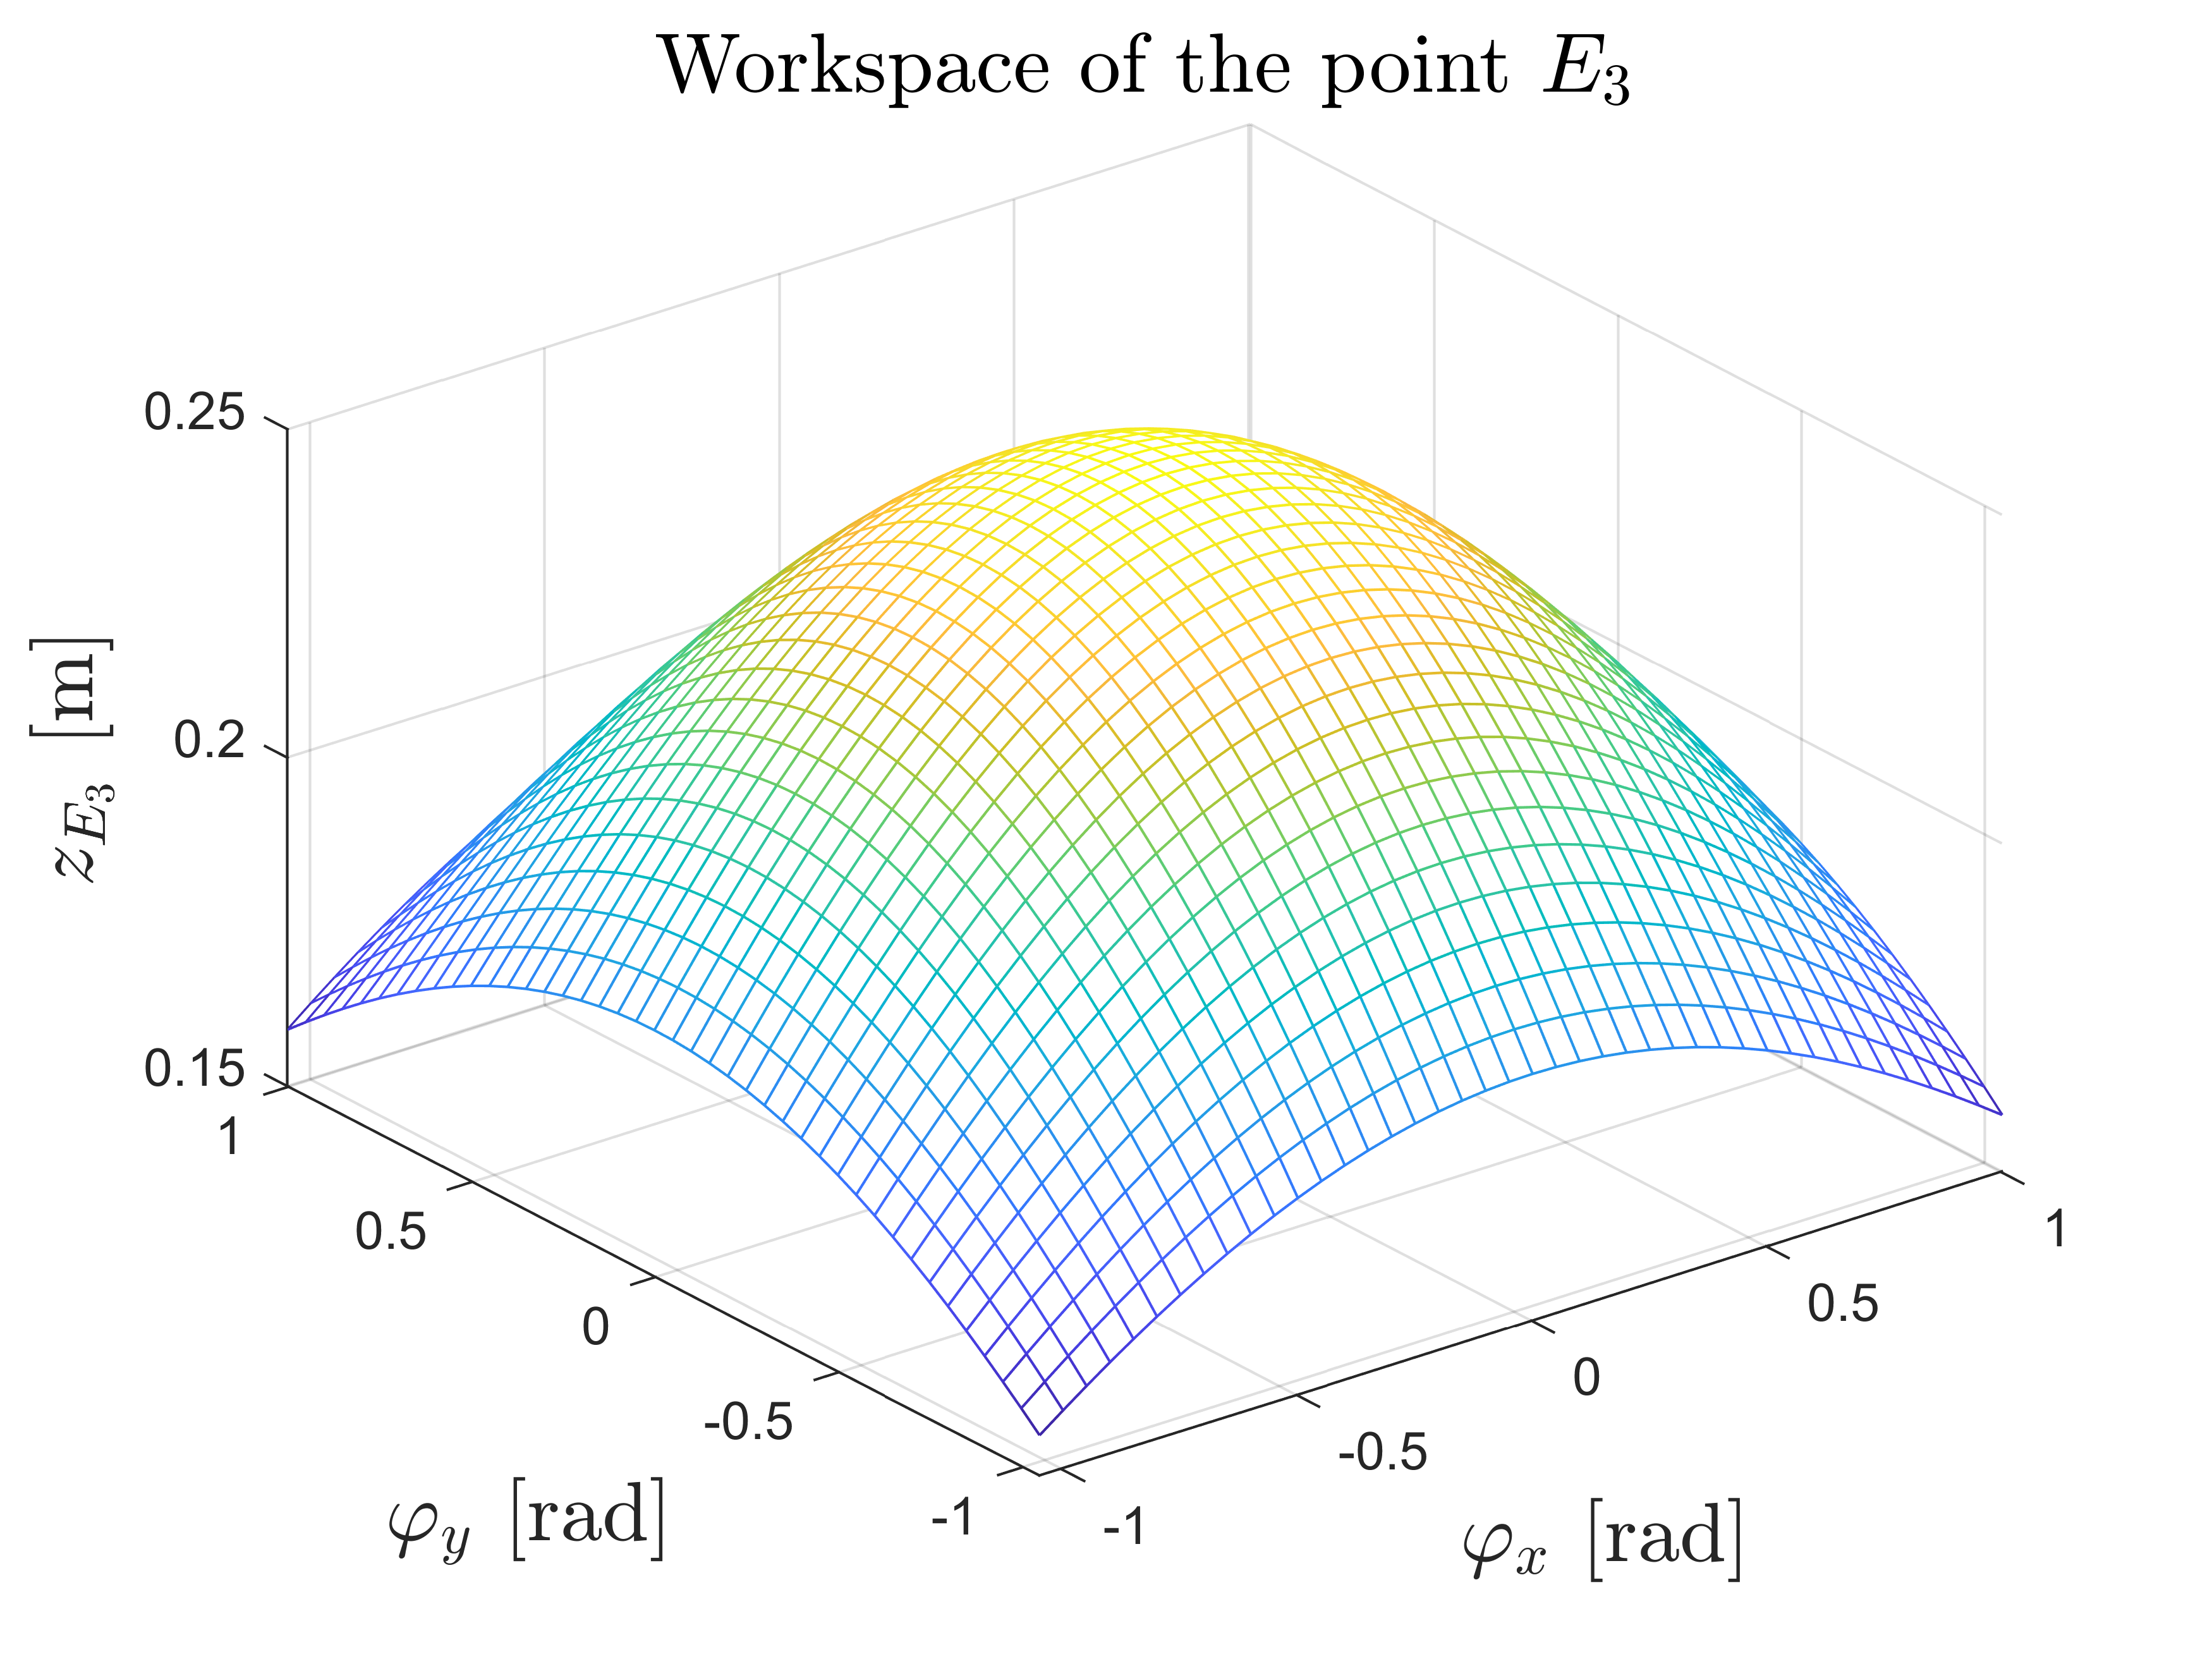
\includegraphics[width=8cm]{figures/Workspace_z_E3_fix_fiy.png}
    \caption{Workspace of the end-point $E_3$ in rotations.}
    \label{fig:E2_rotations}
\end{figure}

\begin{figure}
    \centering
    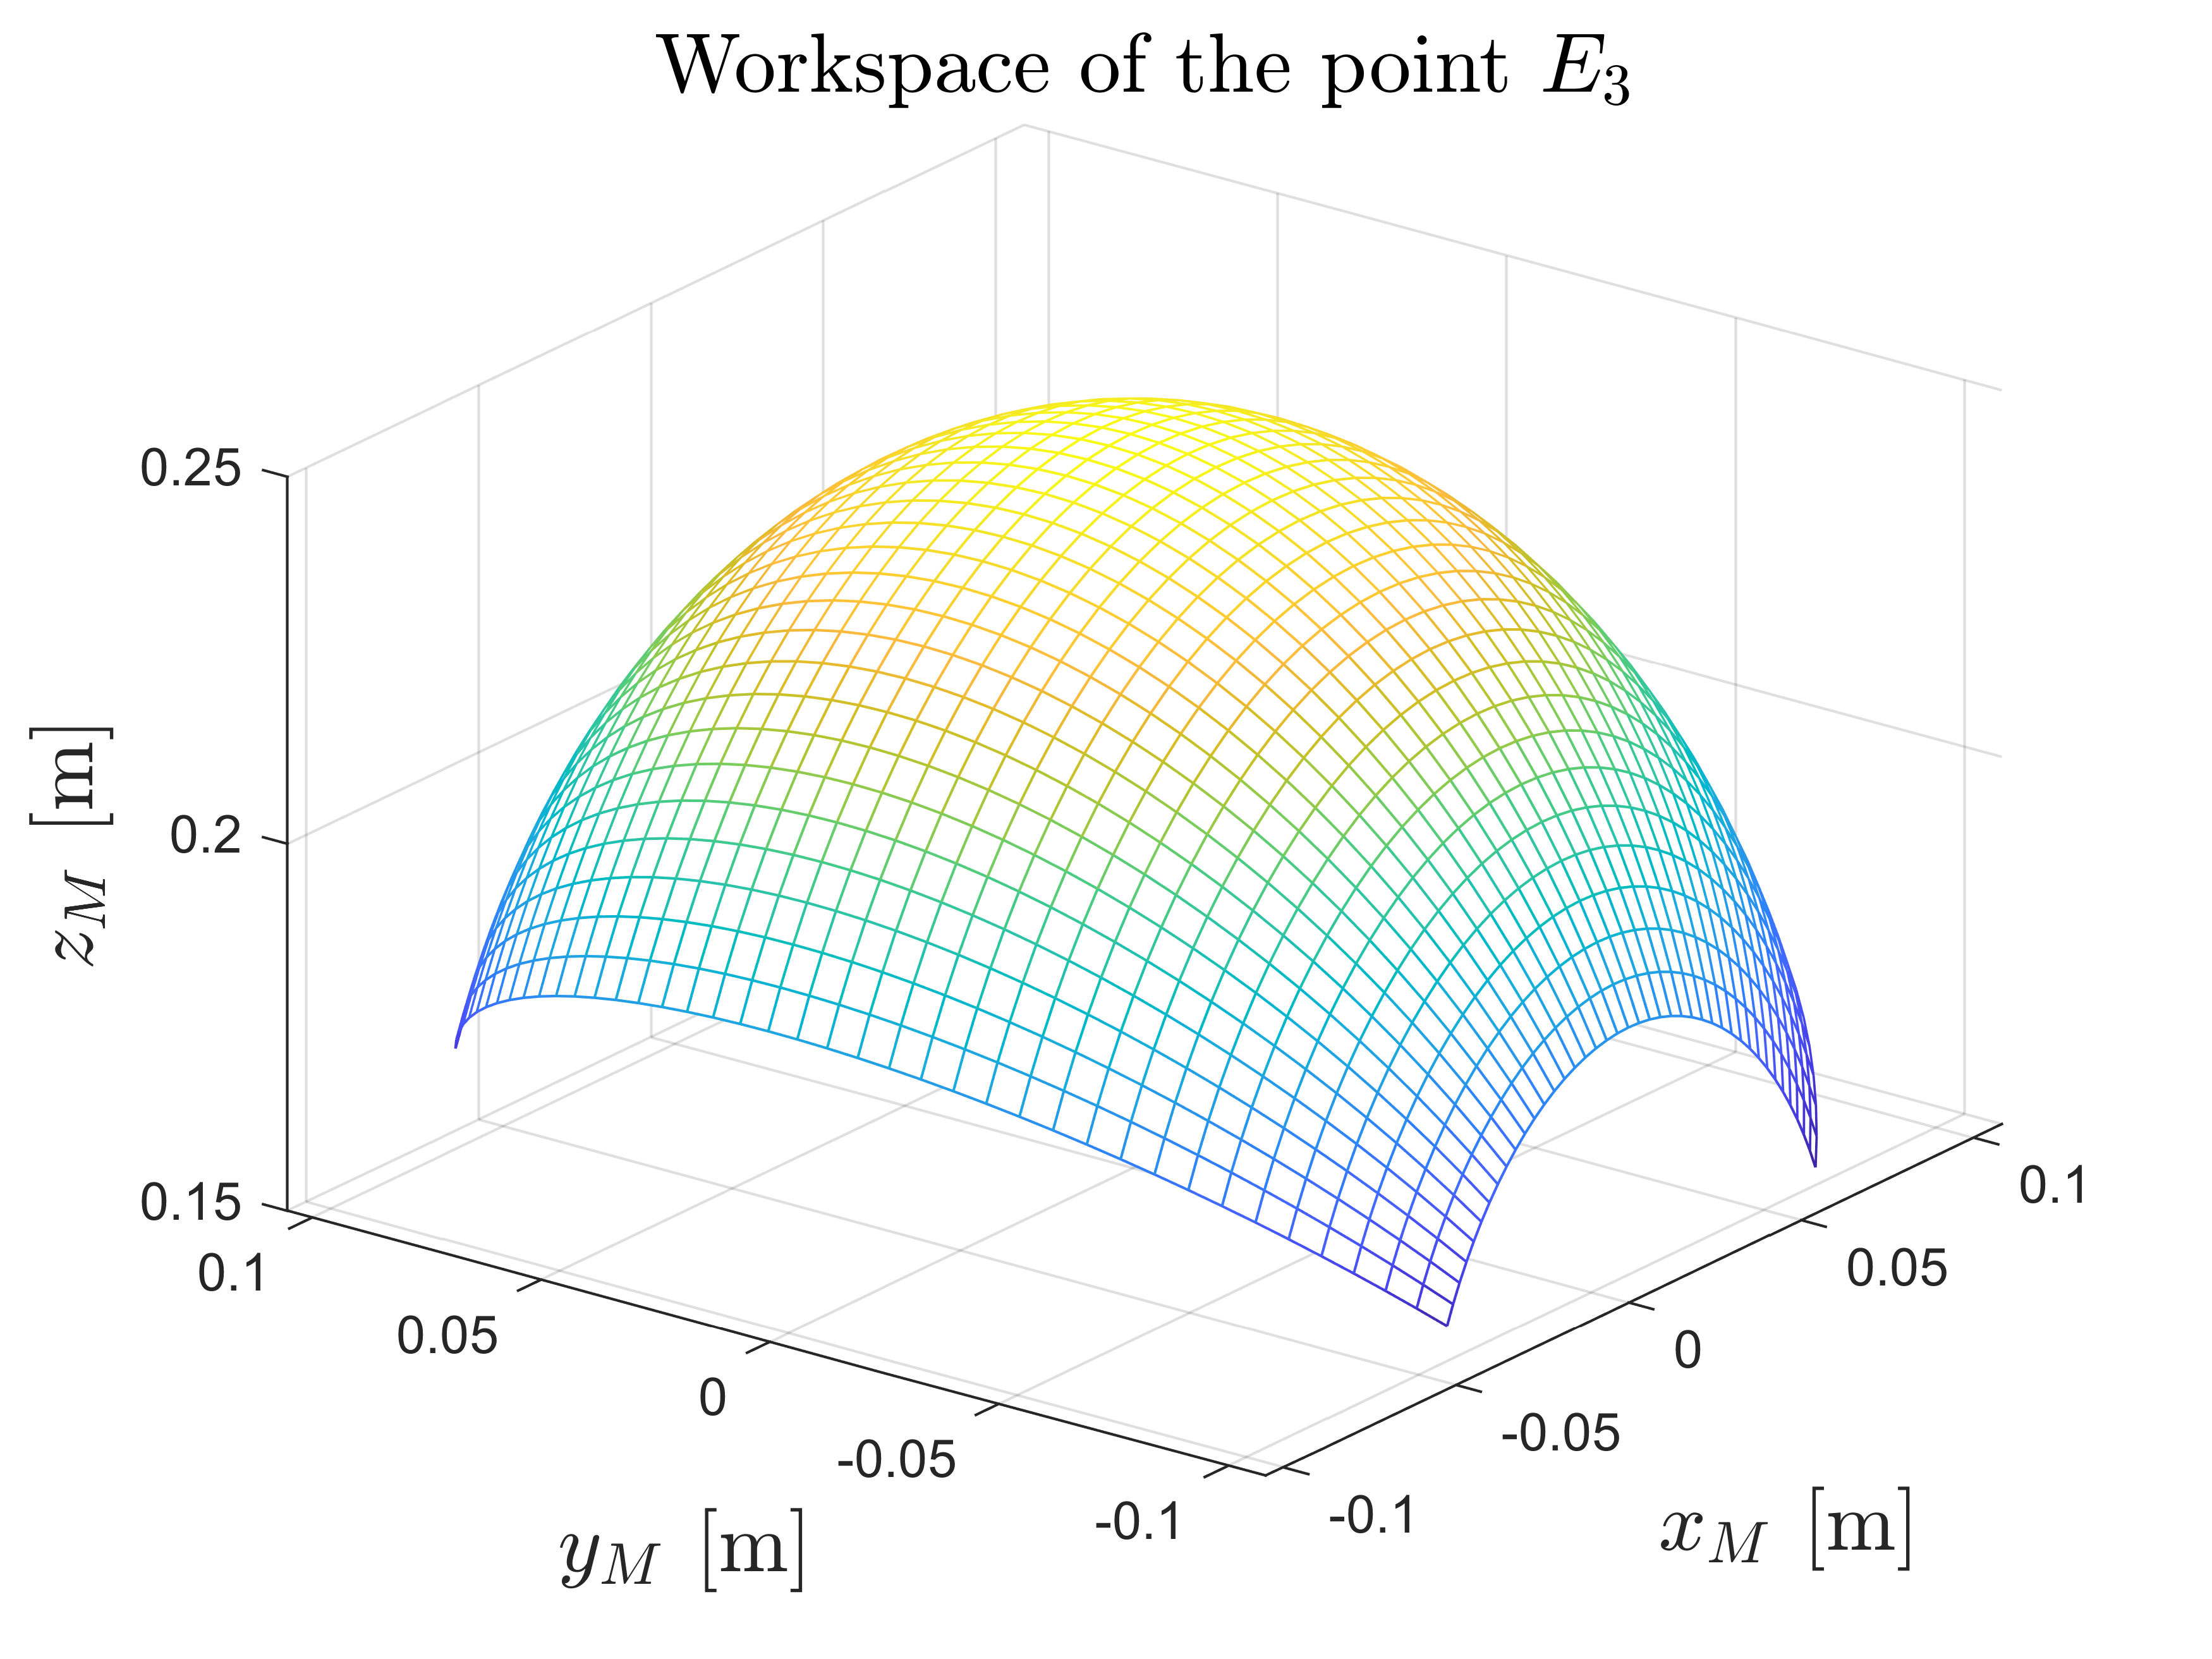
\includegraphics[width=8cm]{figures/Workspace_z_E3_x_y_z.png}
    \caption{Workspace of the end-point $E_3$ in physical coordinates.}
    \label{fig:E2_physical_coordinates}
\end{figure}

In order to investigate the stiffness of the tensegrity joint in the workspace, it is first necessary to set up the equations of force balance and let the system settle in the equilibrium position (form finding, \cite{Ref_Hajzman_OWN_planning_method}, \cite{Ref_Krivosej_OWN_tensegrity_based_robots}). However, for a chosen identical prestress in all cables (200 N chosen), we do not obtain the exact desired position. This new steady state position depends on the specific position in the workspace.

To obtain the stiffness of serial robots and kinematic structures, it is common to load the end-effector with a force or moment \cite{Ref_Jubien_STIFFNESS_Identicication_KUKA}, \cite{Ref_Dumas_STIFFNESS_identicication_serial_robots}, or a combination thereof, and then determine the resulting stiffness from the deformation \cite{Ref_Palli_STIFFNESS_Joint_var_stiffness}, \cite{Ref_Dumas_STIFFNESS_stiffness_identification_6dof}. 

To investigate the stiffness of the tensegrity joint, the endpoint E3 of the structure was loaded with a force or moment in the steady state. Subsequently, the strain was subtracted and the stiffness was calculated from the obtained deformation. The tensegritic revolute joint was loaded by the force in the $z$ direction of movement (Fig.~\ref{fig:revolute_joint_stiffness_z_axis}). The stiffness for the revolute joint is calculated for half of the range, since the stiffness is symmetrical.

\begin{figure}
    \centering
    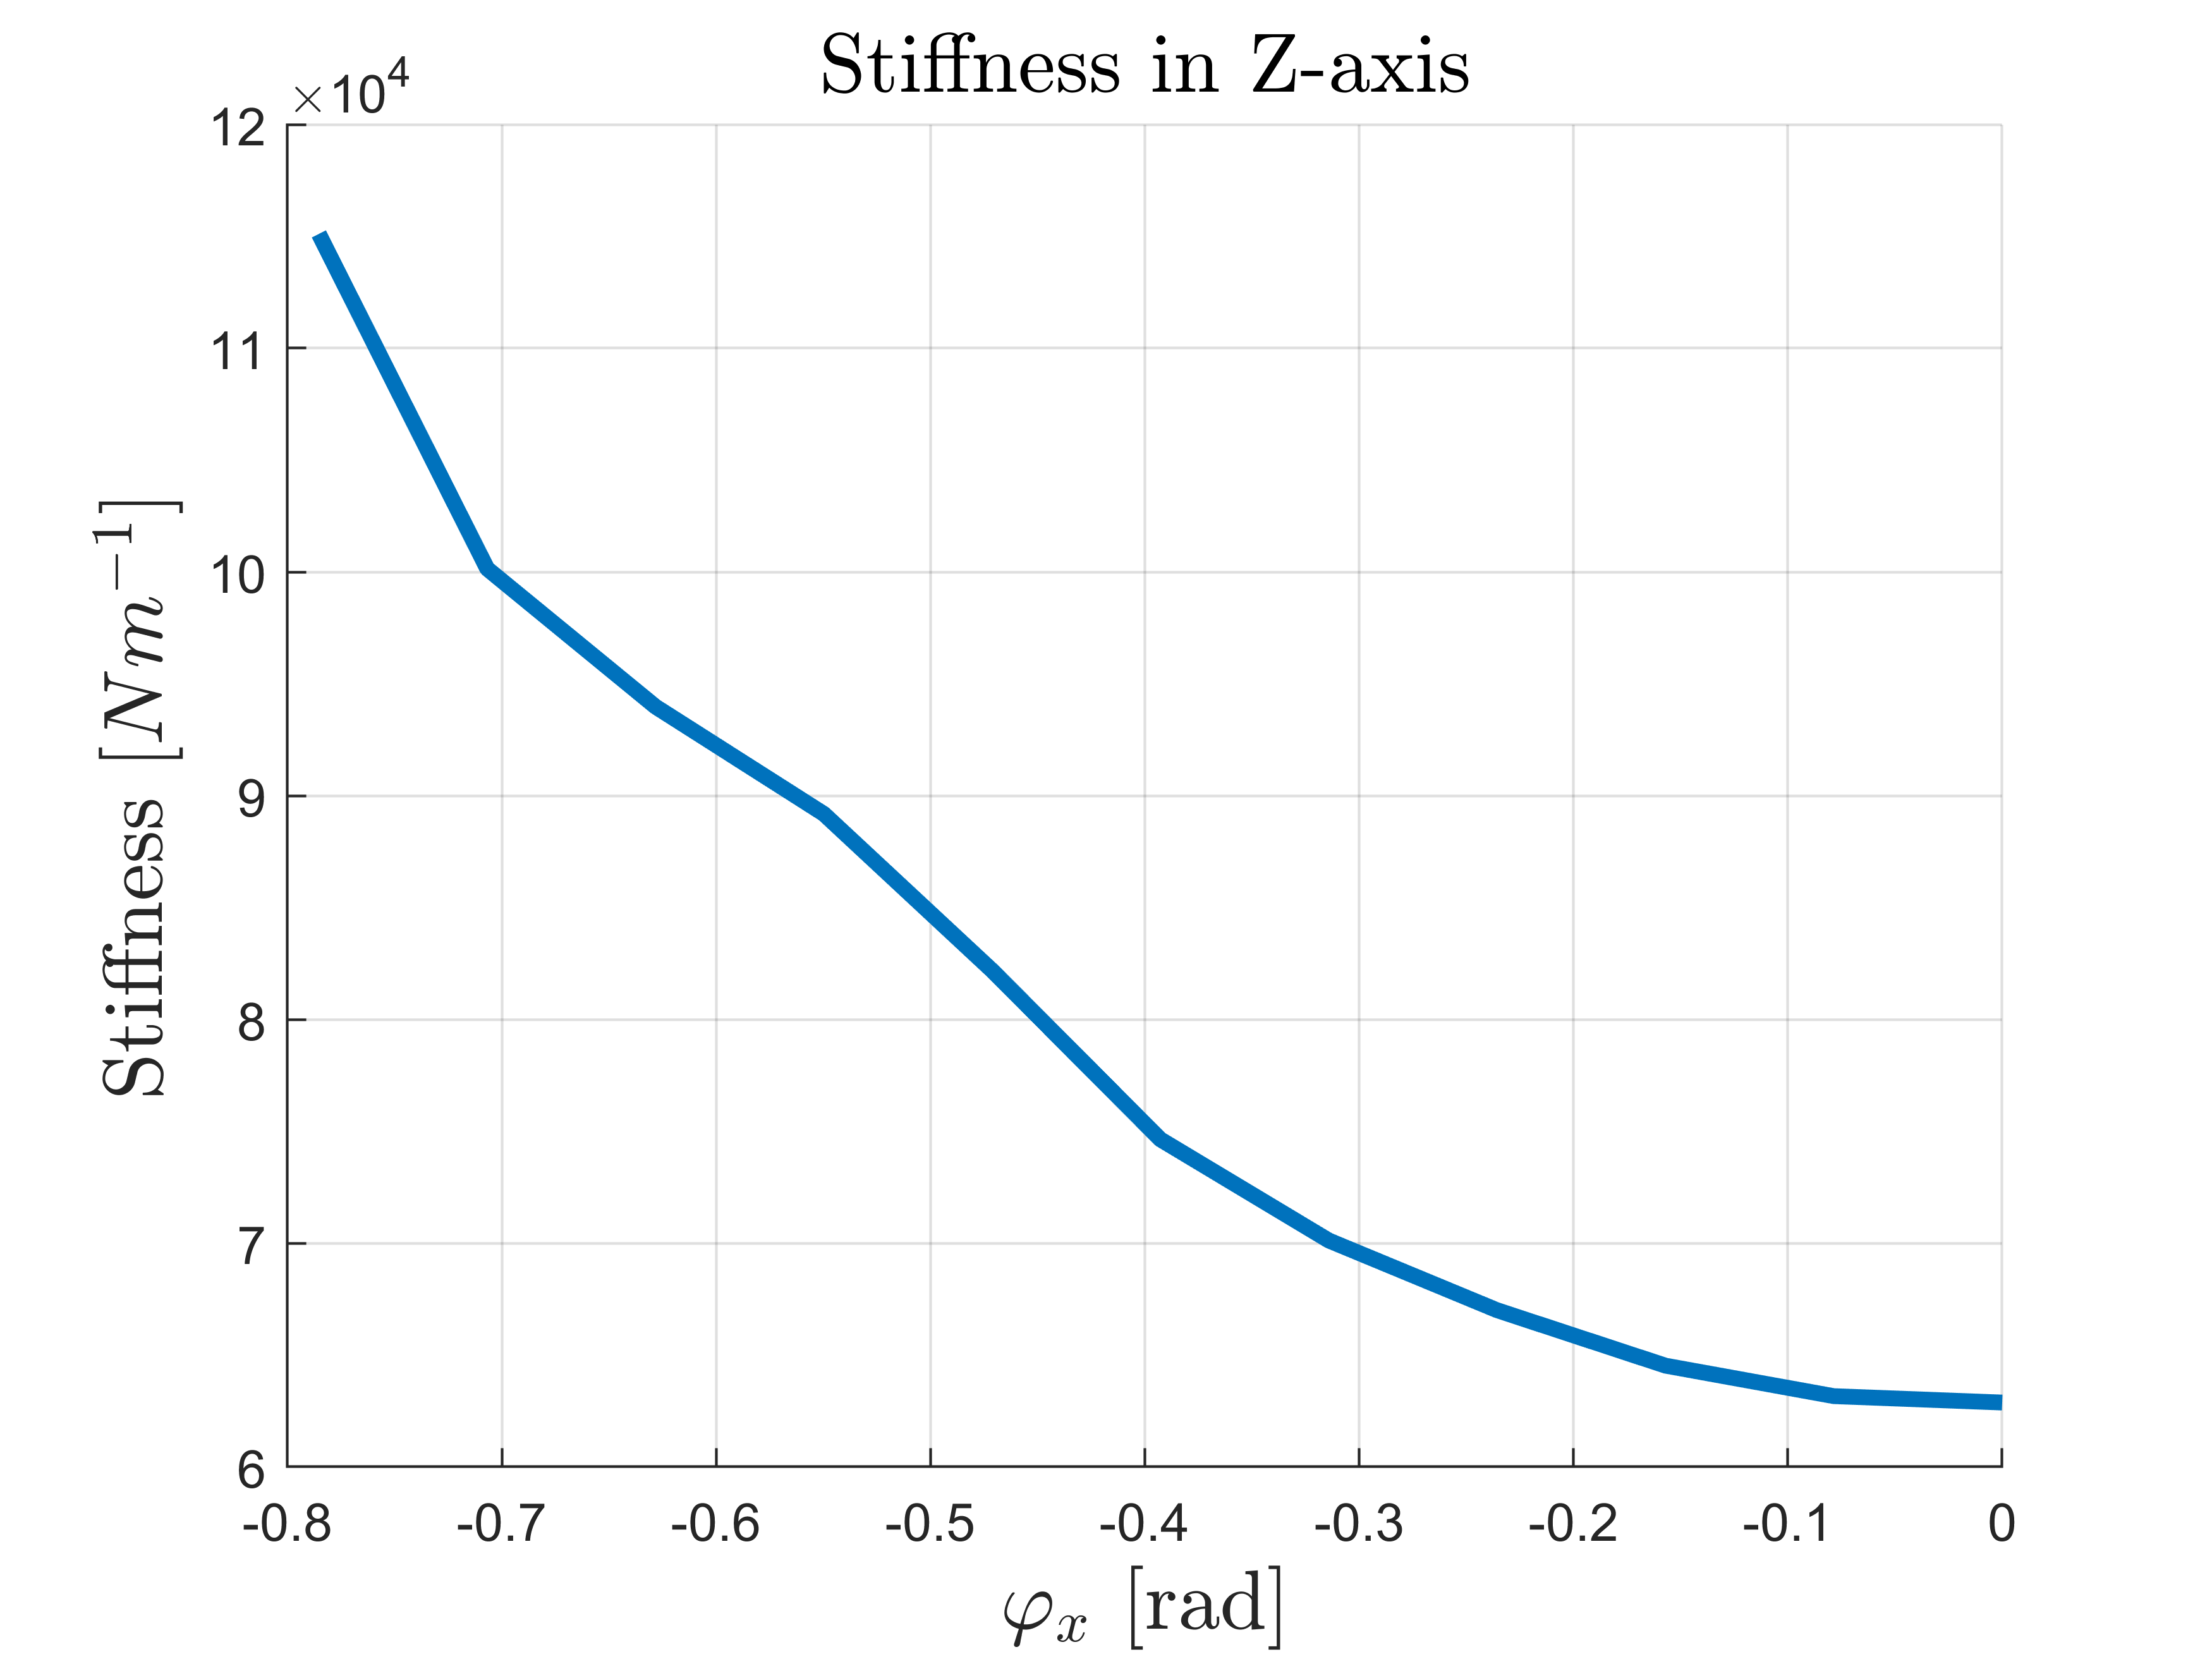
\includegraphics[width=8cm]{figures/revolute_joint_stiffnes_Z.png}
    \caption{Stifness in z-axis of the revolute joint for z-axis force load. }
    \label{fig:revolute_joint_stiffness_z_axis}
\end{figure}

\begin{figure}
    \centering
    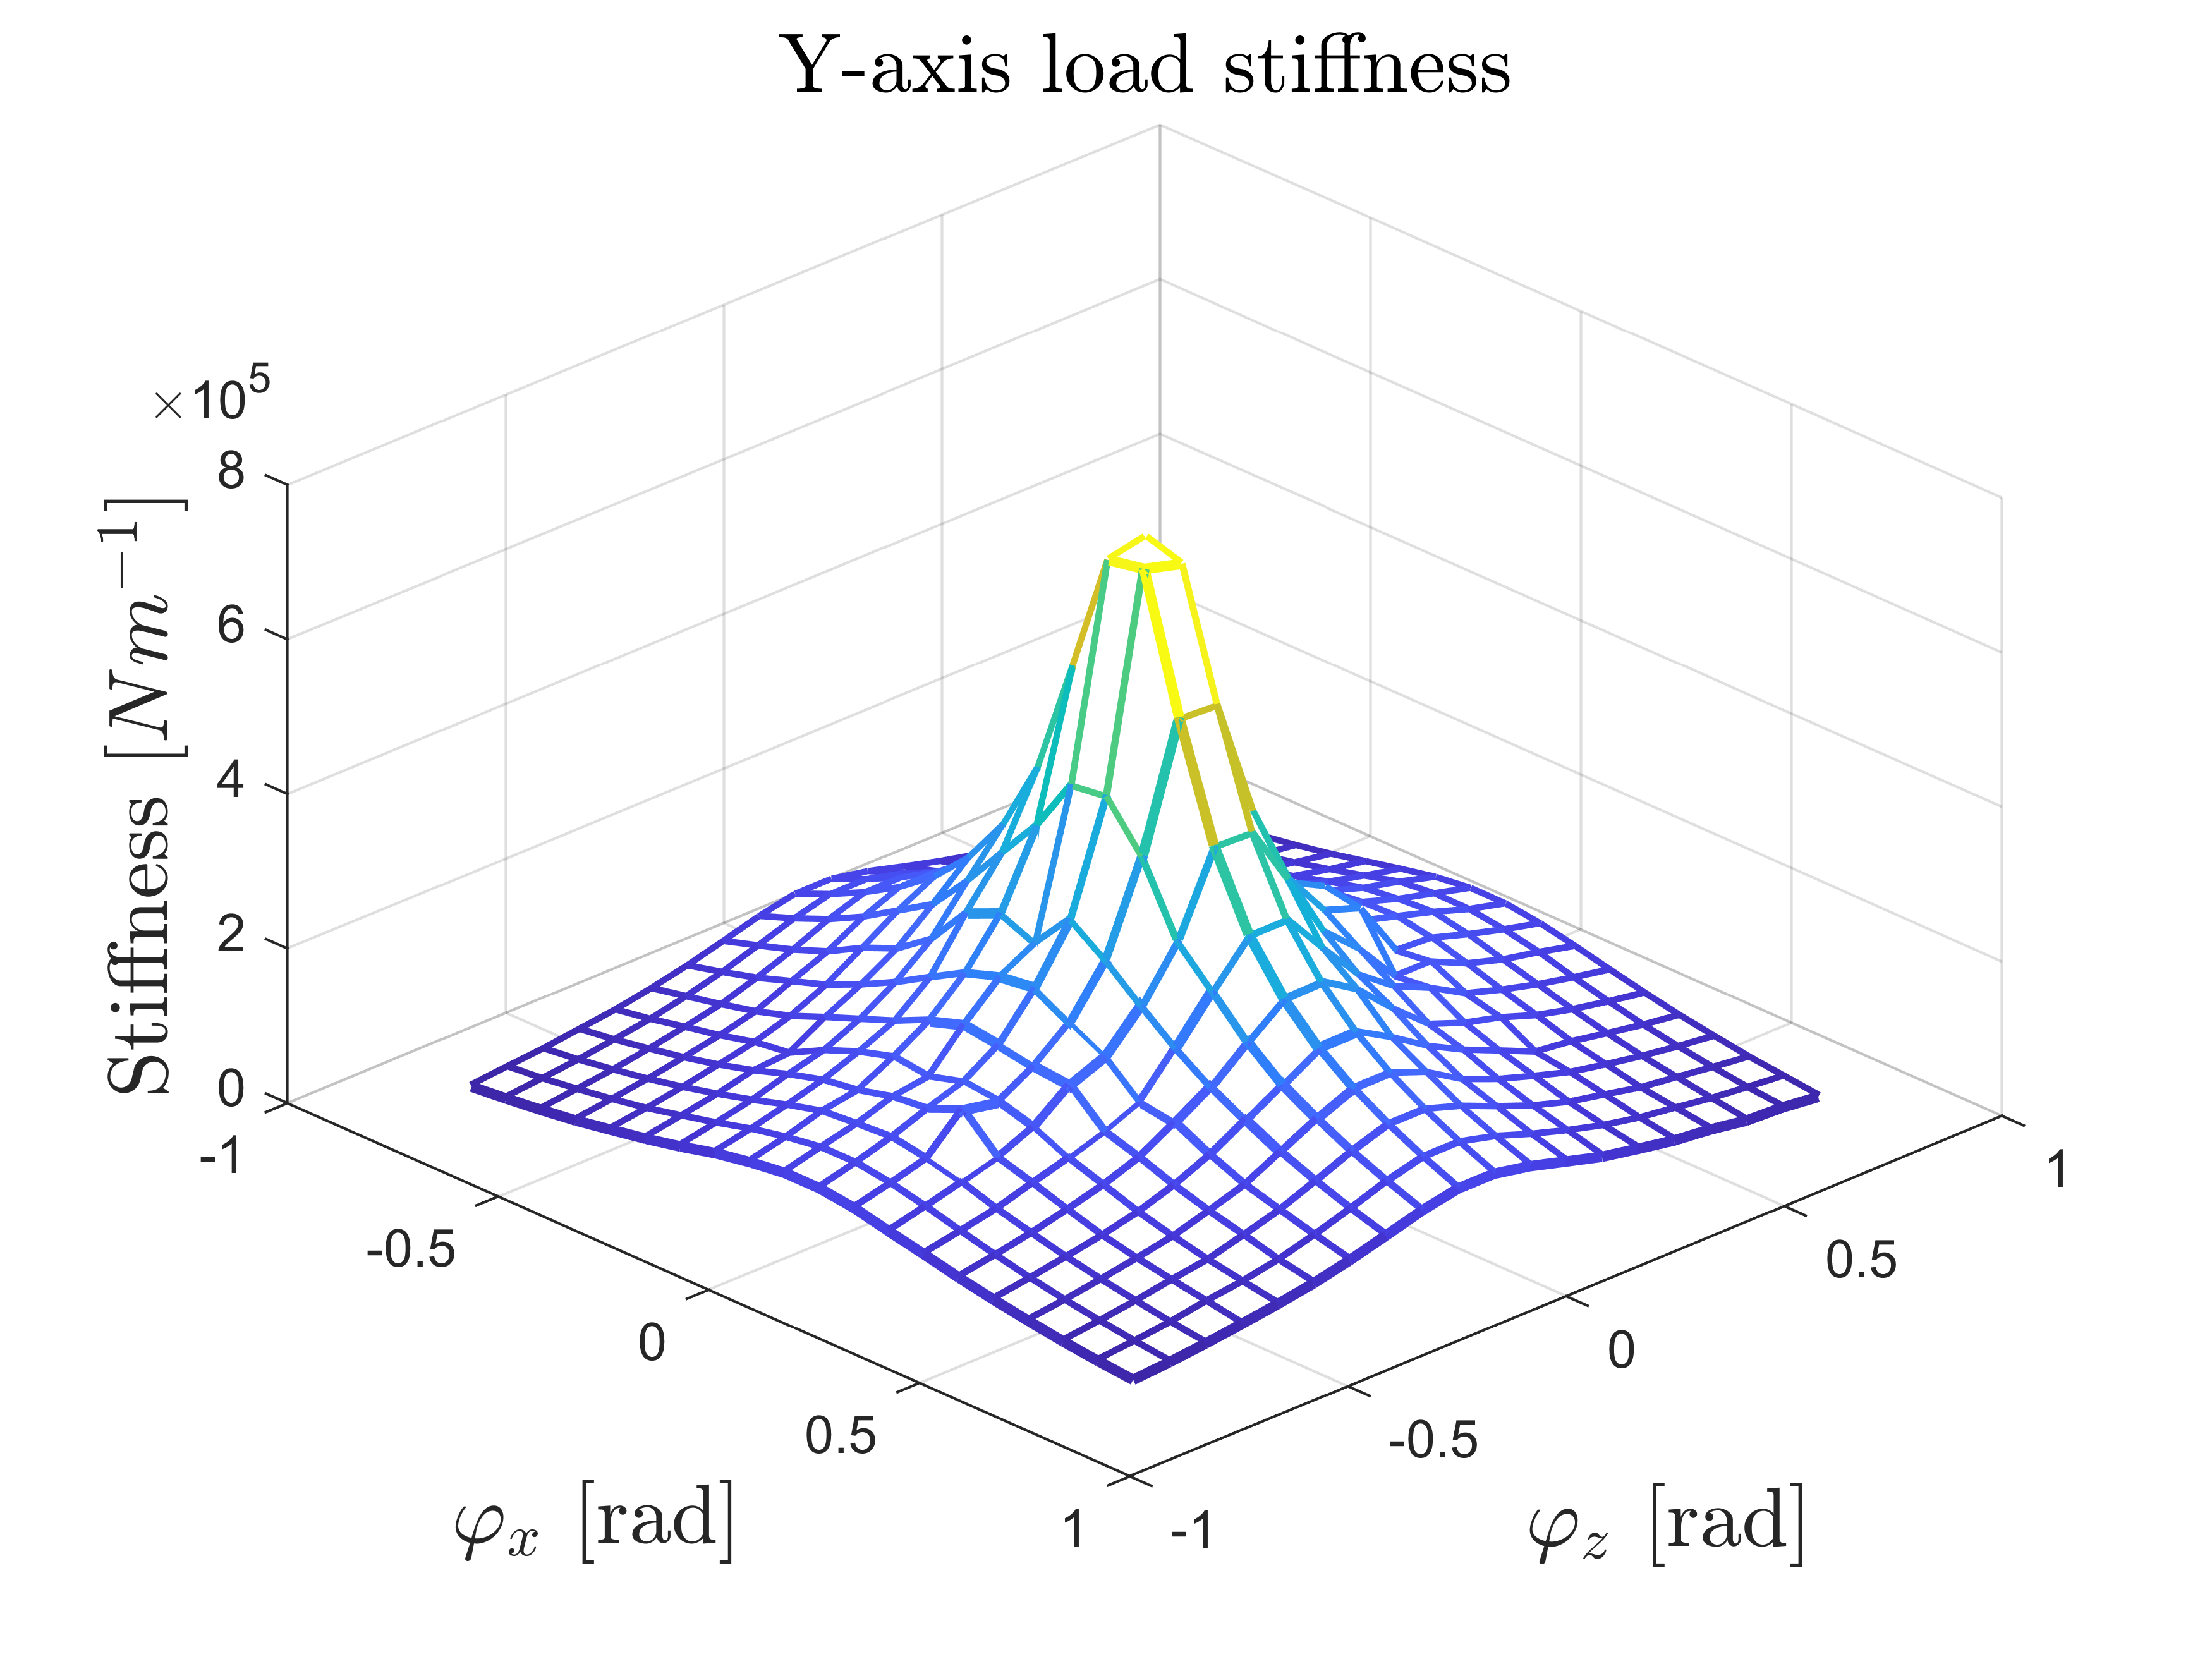
\includegraphics[width=8cm]{figures/universal_joint_Fy_load.png}
    \caption{Stiffness of the universal joint for the $y$ axis force load.}
    \label{fig:universal_joint_Fy}
\end{figure}

\begin{figure}
    \centering
    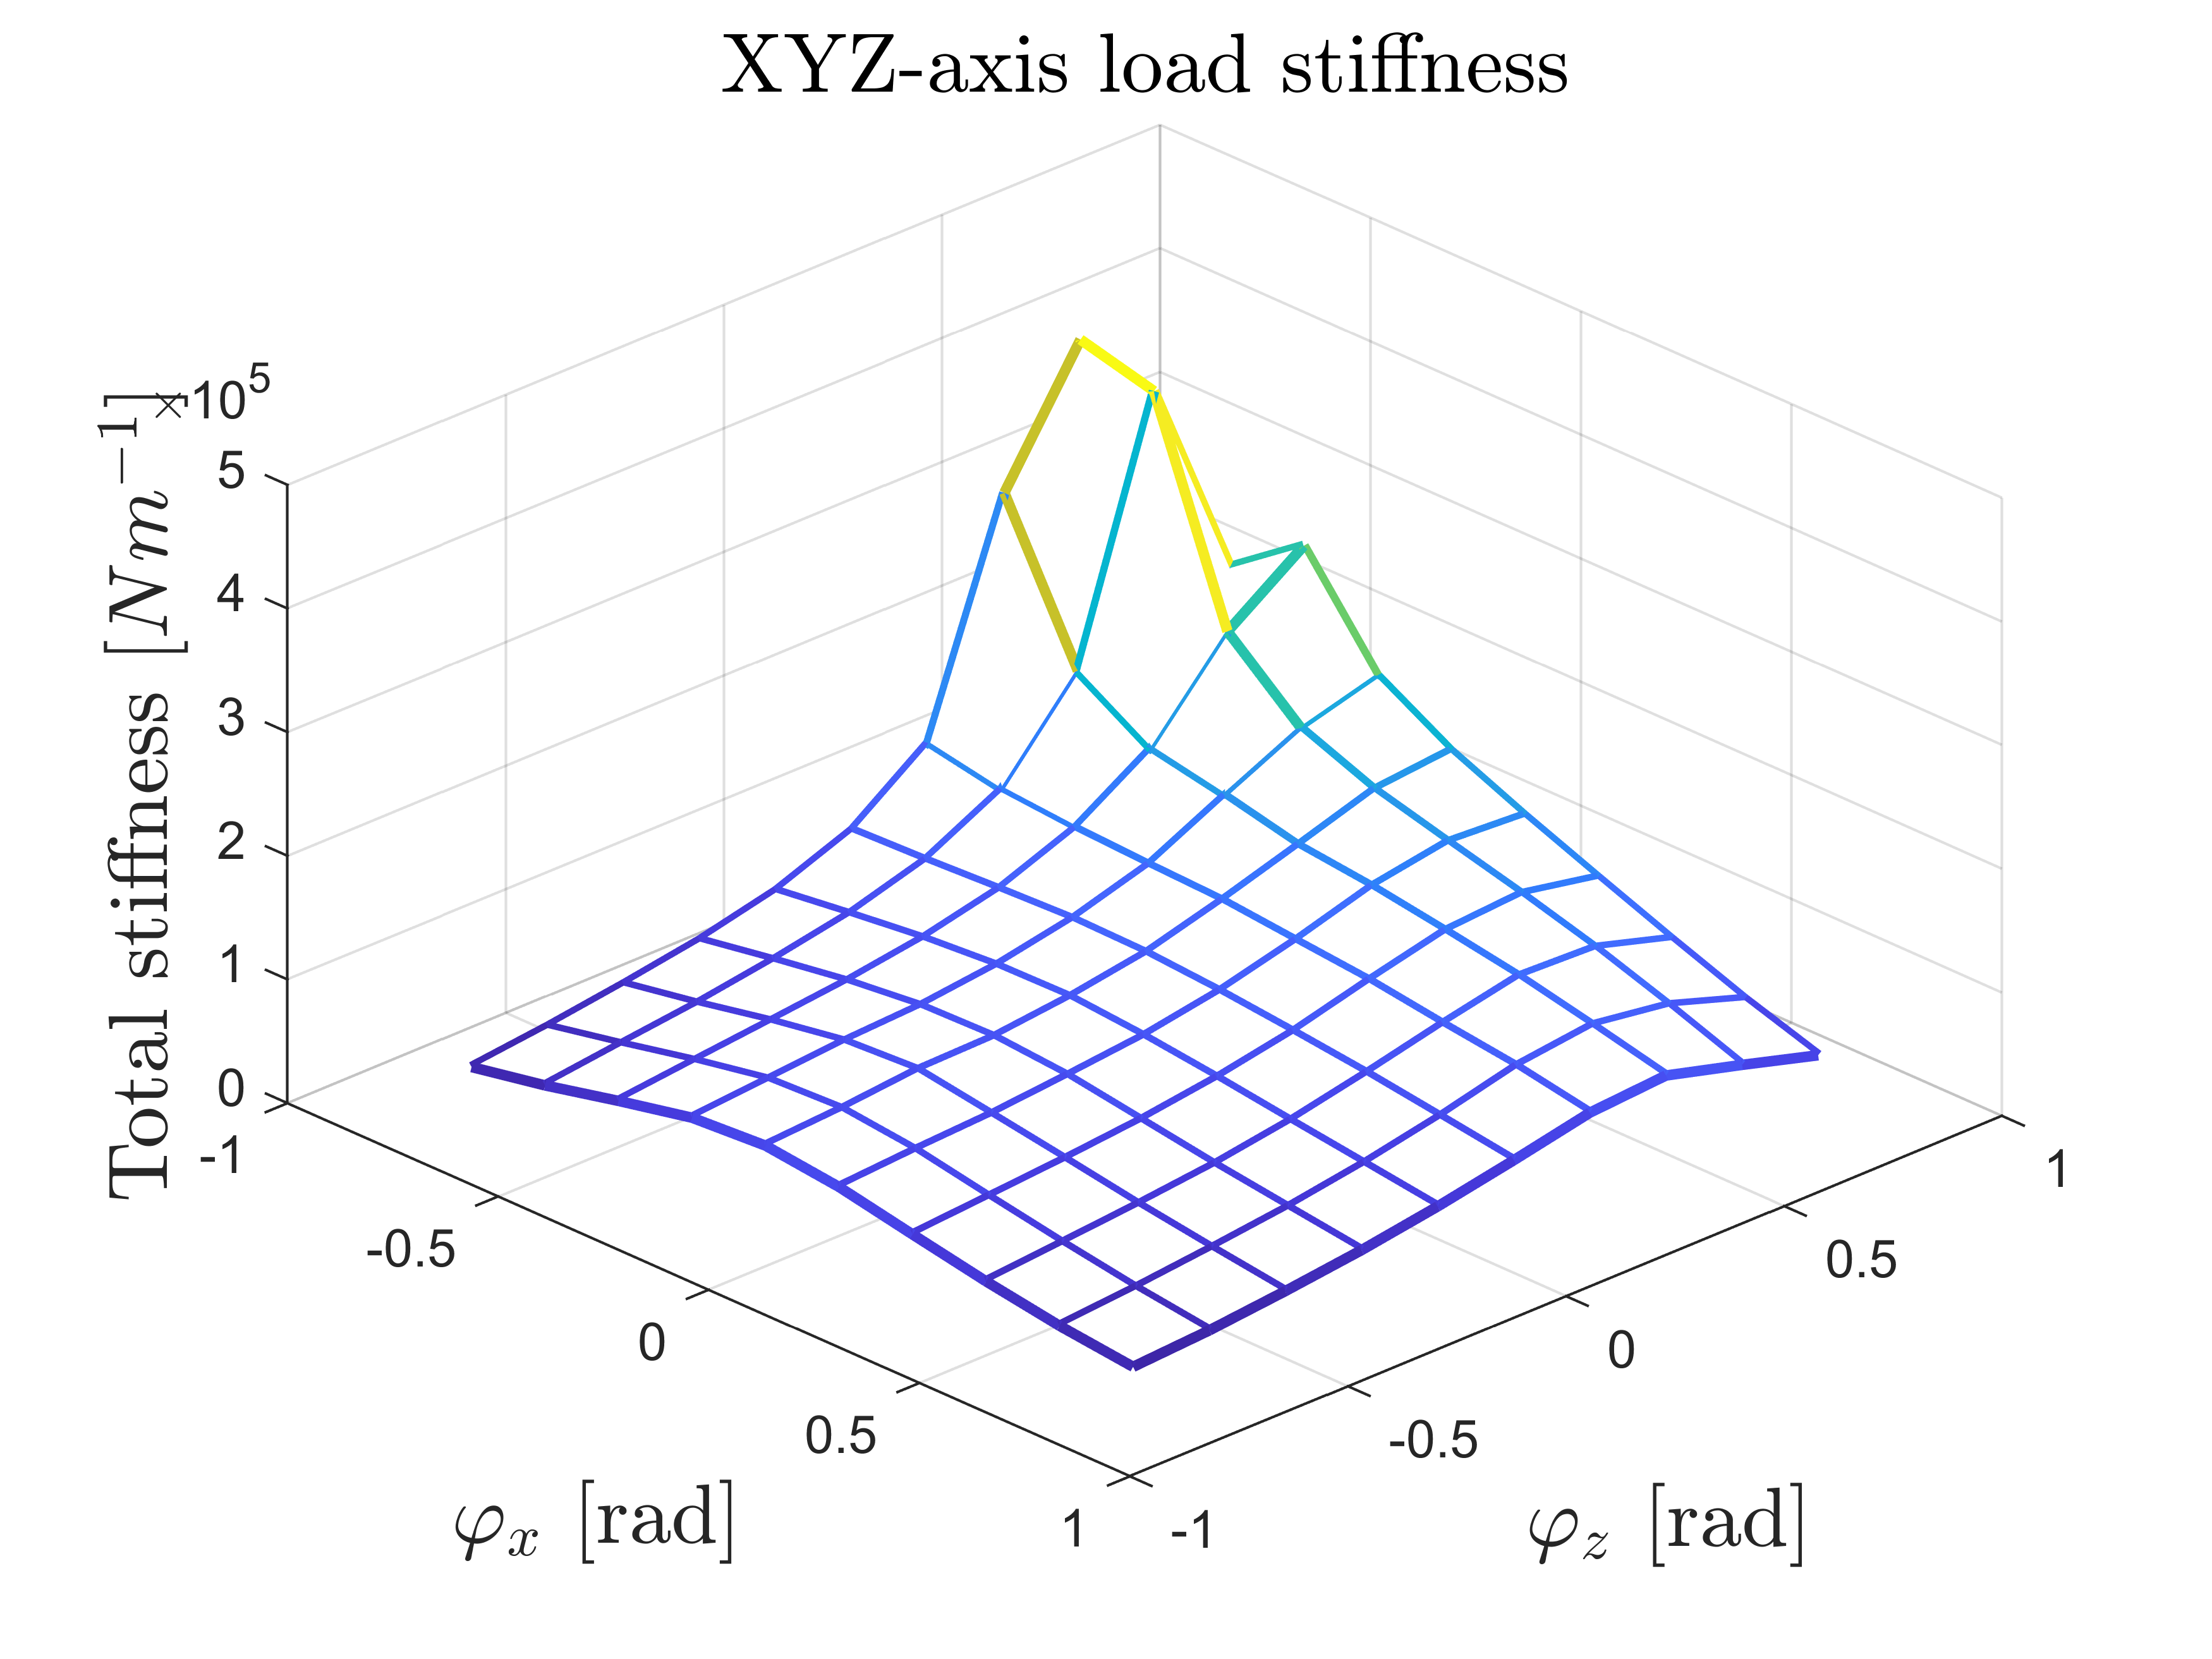
\includegraphics[width=8cm]{figures/universal_joint_Fxyz_load.png}
    \caption{Stiffness of the universal joint for the $x-y-z$ axis force load.}
    \label{fig:universal_joint_Fxyz}
\end{figure}

\begin{figure}
    \centering
    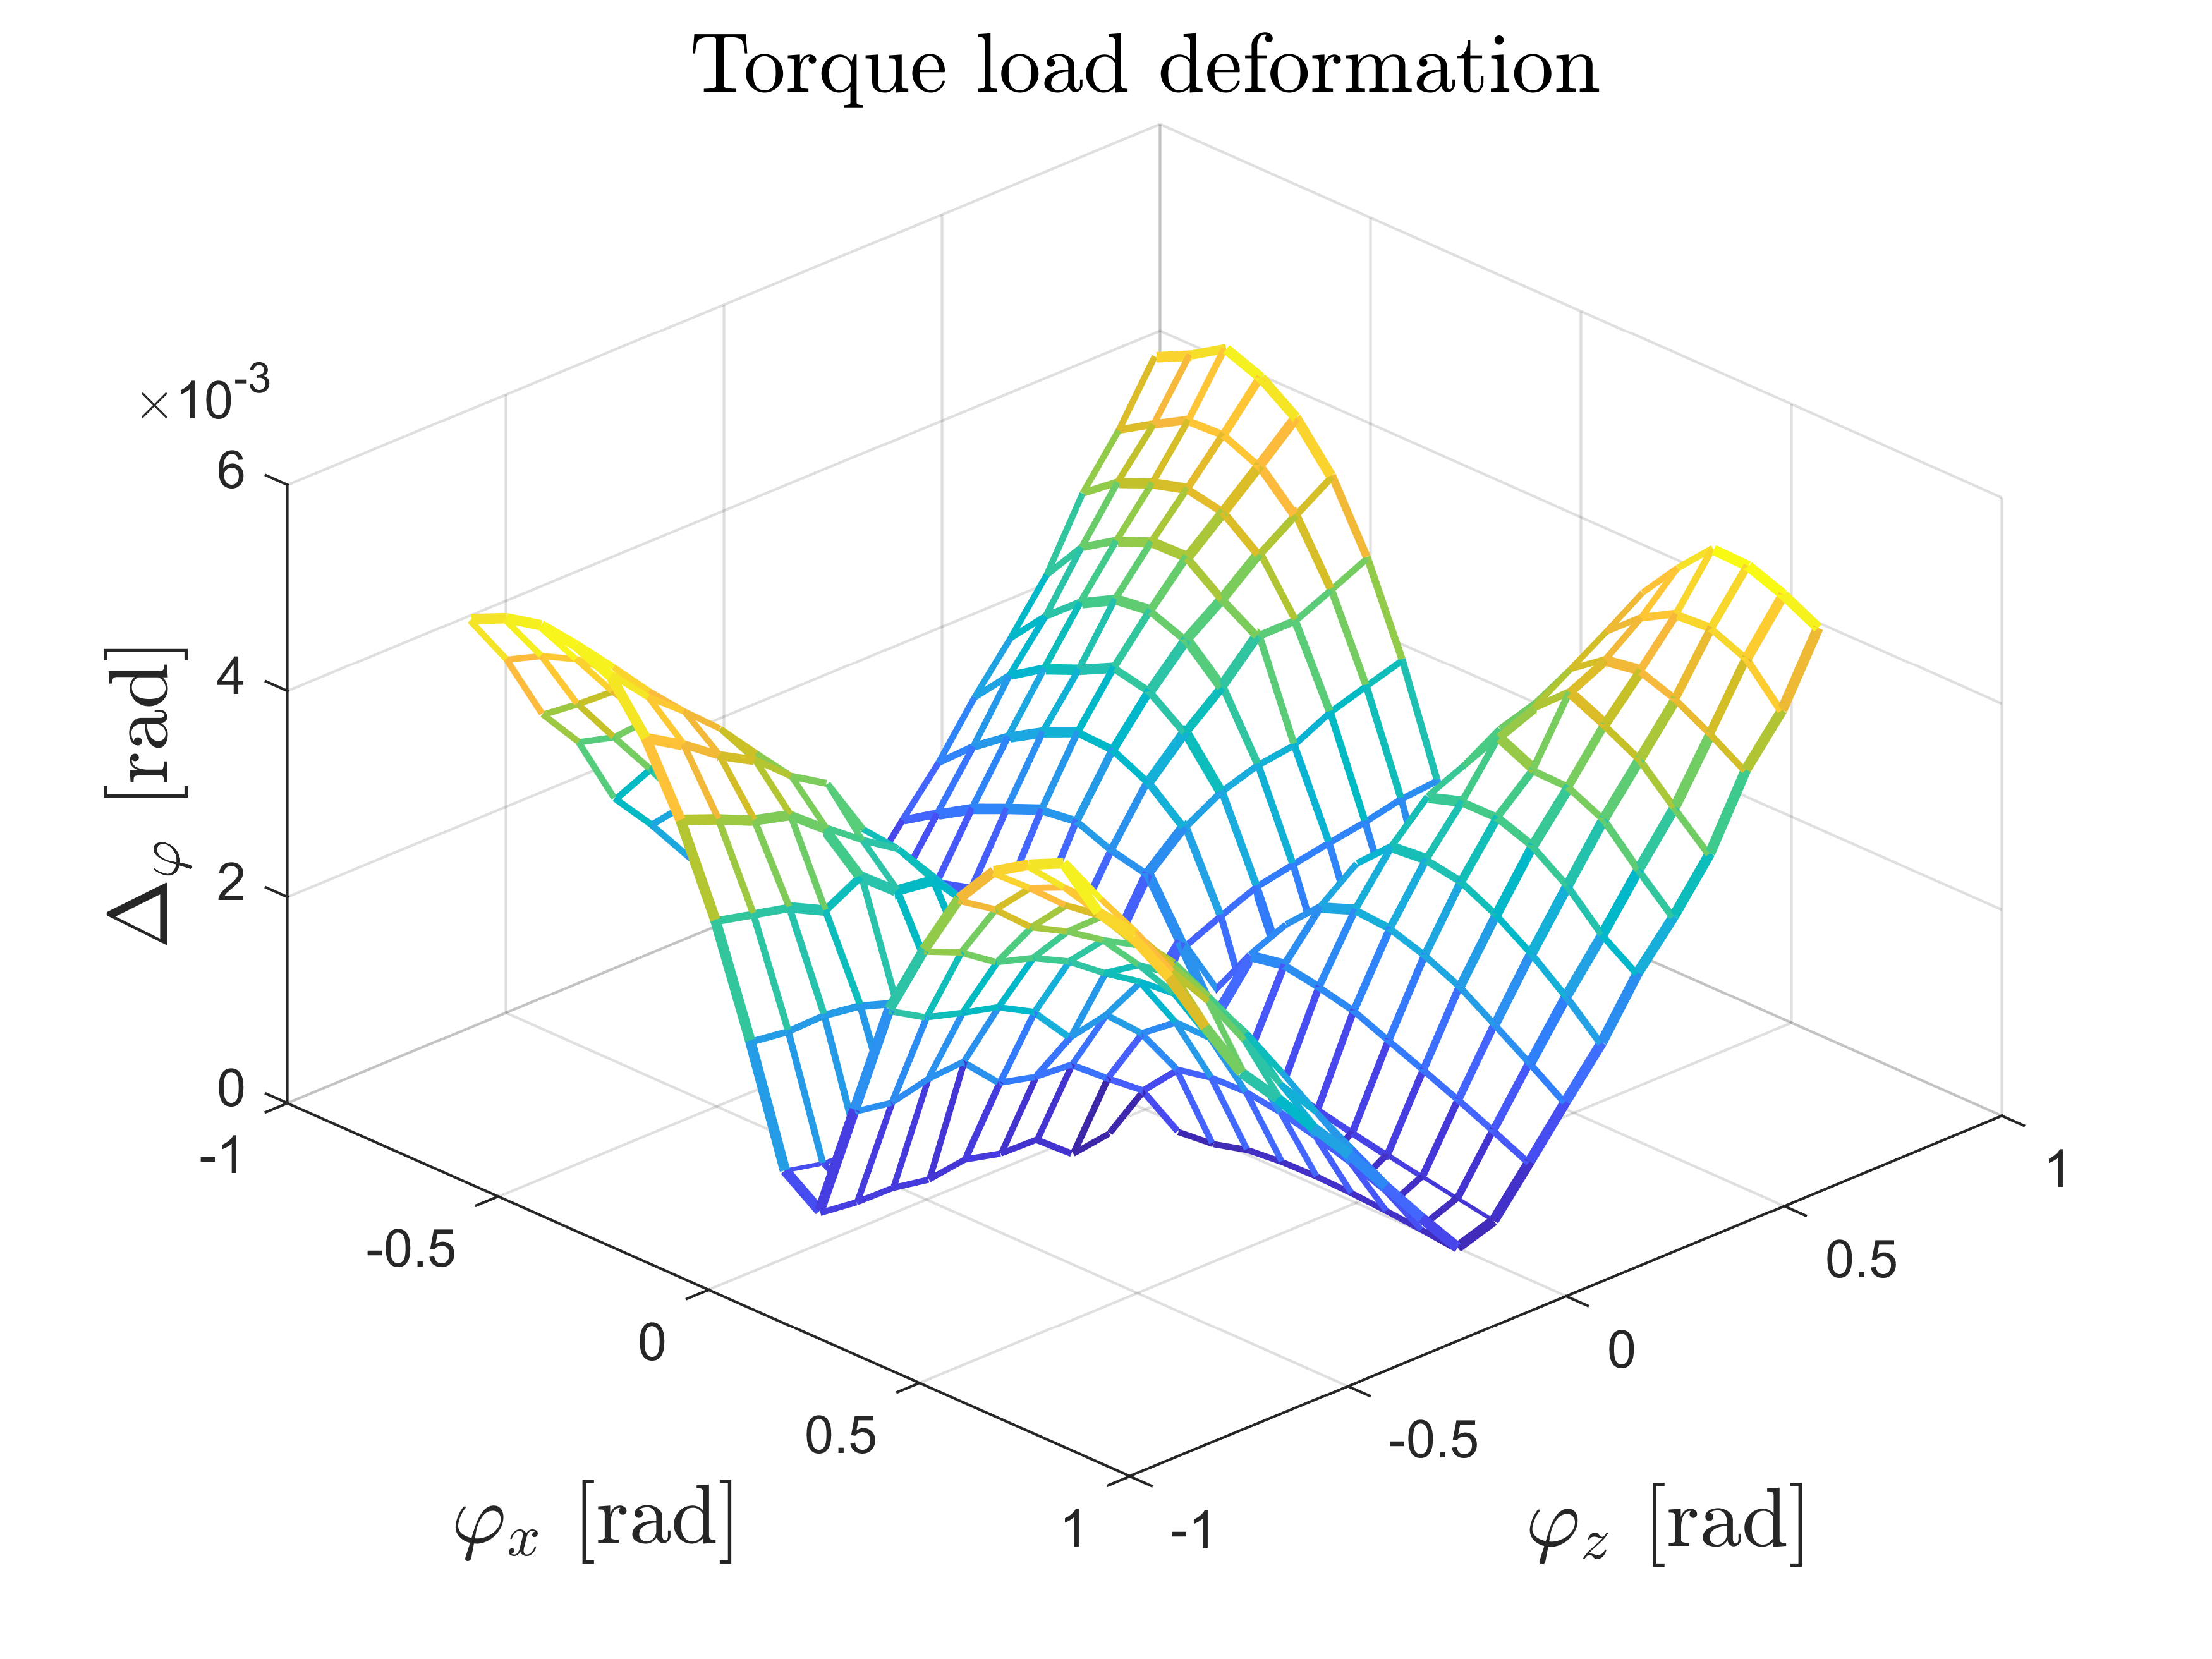
\includegraphics[width=8cm]{figures/universal_joint_torque_load.png}
    \caption{Stiffness of the universal joint for the $y$ axis torque load.}
    \label{fig:universal_joint_My}
\end{figure}

The stiffness of the tensegrity universal joint is calculated for three cases. The first case is the loading of the point $E_3$ in the y-axis (Fig.~\ref{fig:universal_joint_Fy}). The second case is the loading of point $E_3$ by the same force components in the $x$, $y$ and $z$ directions (Fig.~\ref{fig:universal_joint_Fxyz}.) The third case is for loading the body at point E3 with a torque in the y-axis direction (Fig.~\ref{fig:universal_joint_My}).


\subsection{Experiment}

In order to verify the functionality of the proposed tensegrity joint, a model was created using FDM 3D printing, fasteners and cables. The model (Figs.~\ref{fig:CAD_model_upper_part} and \ref{fig:CAD_model_bottom_part}) is created according to the design in Fig.~\ref{fig:revolute_universal_joint}. he dimensions are chosen in agreement with the simulations and stiffness calculations.

The tensegrity joint system consists of two bodies and six cables. The cables marked $c_1$ and $c_2$ are parts of a single drive cable leading from point $V_2$ through points $B_2$ and $A_2$ to point $U_2$. Between points $A_2$ and $B_2$ is a pulley through which the cable is guided and actuated. The same drive principle is used with cables $c_7$ and $c_8$. This time the drive cable is led from point $A_3$ through $U_2$ and $V_2$ to the point $B_3$. 

\begin{figure}
    \centering
    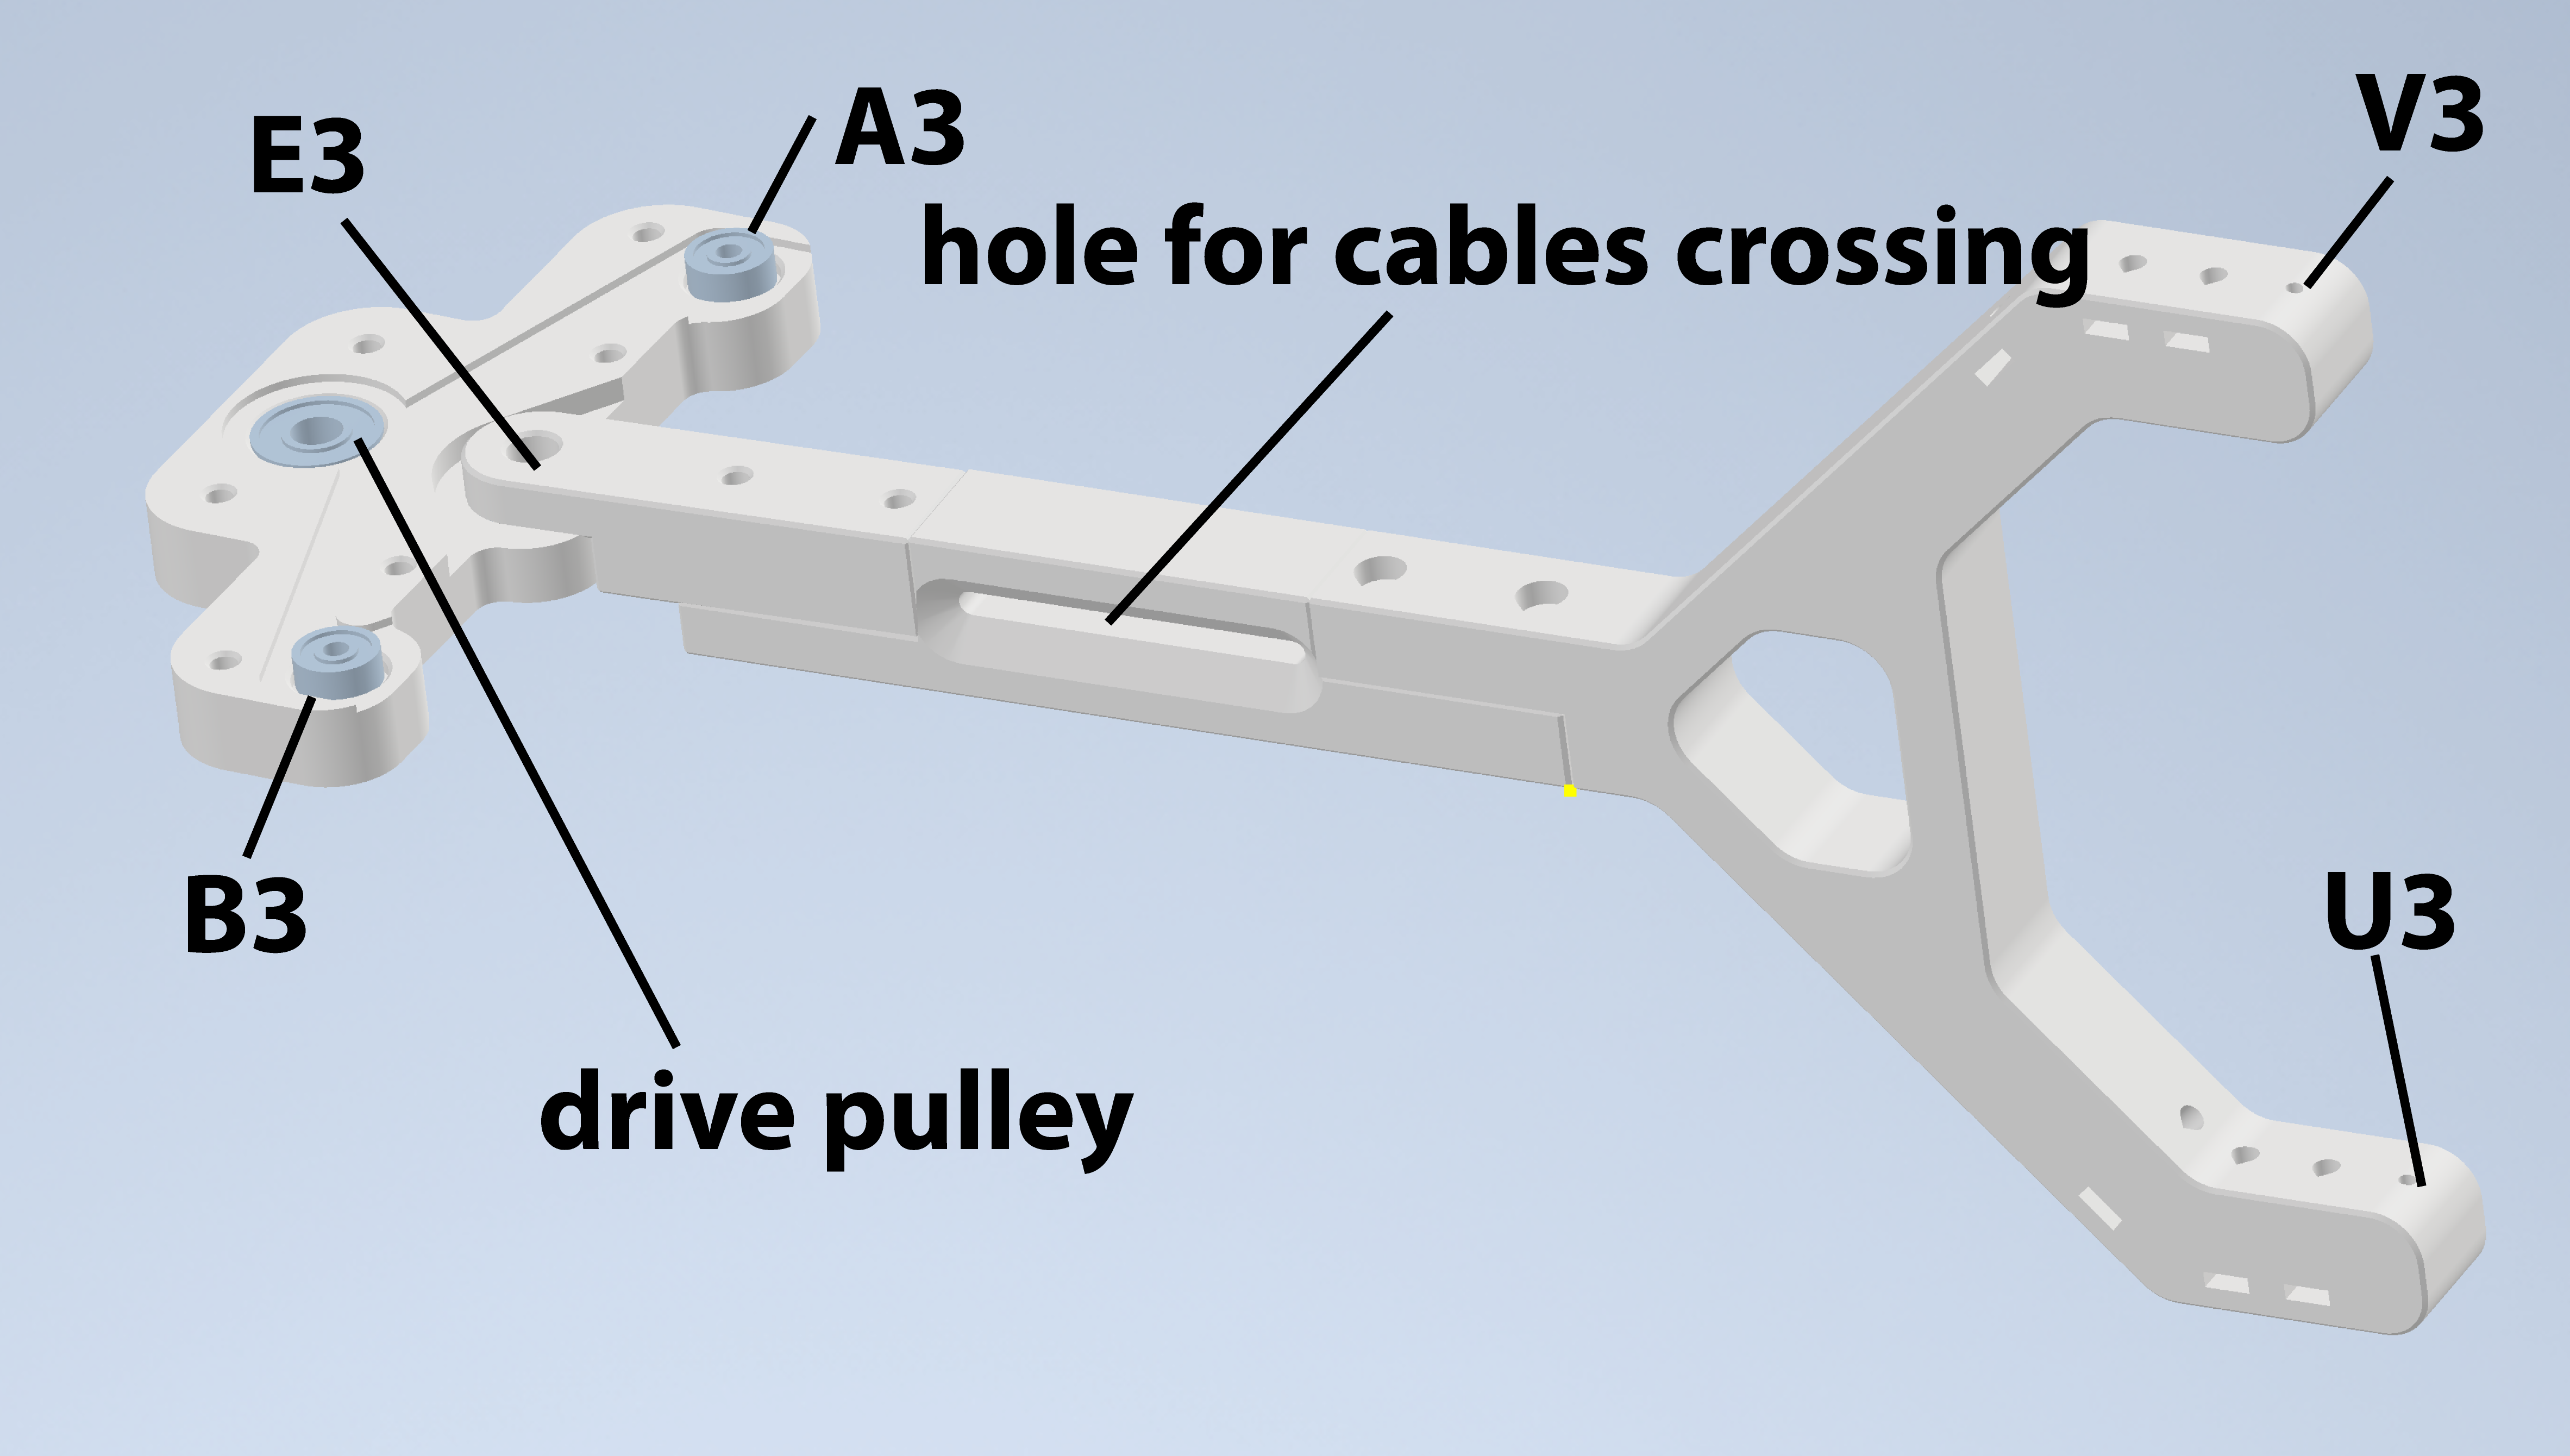
\includegraphics[width=12cm]{figures/tensegrity_revolute_joint_fixed_top_modif_AI.png}
    \caption{CAD model of the upper part of the tensegrity joint.}
    \label{fig:CAD_model_upper_part}
\end{figure}

\begin{figure}
    \centering
    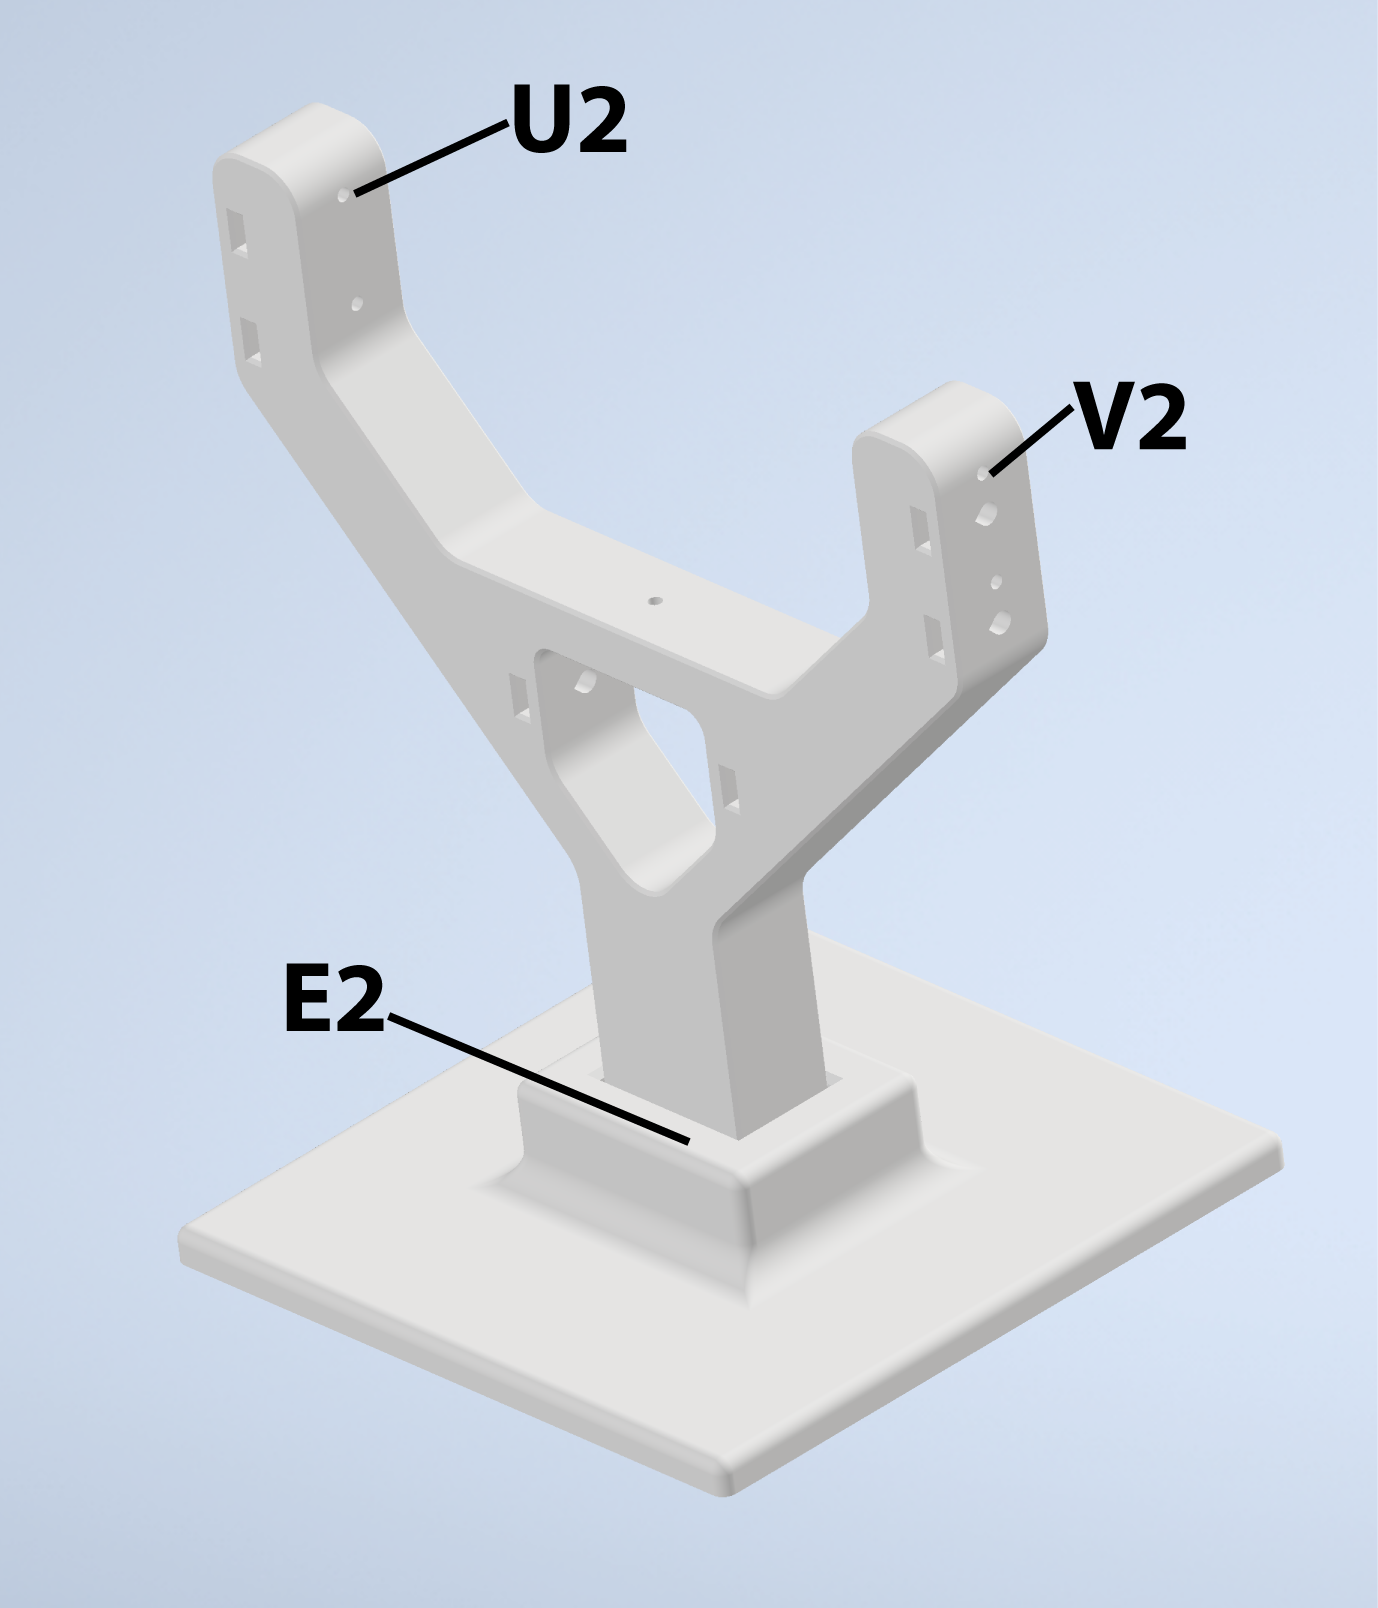
\includegraphics[width=7cm]{figures/tensegrity_revolute_joint_fixed_bottom_modif_AI.png}
    \caption{CAD model of the bottom part of the tensegrity joint.}
    \label{fig:CAD_model_bottom_part}
\end{figure}

\begin{figure}
    \centering
    \includegraphics{}
    \caption{Resulting model}
    \label{fig:resulting_model}
\end{figure}


The resulting constructed model is shown in the Fig.~\ref{fig:resulting_model}. The picture shows a tensegrity rotary link driven by a servomotor via a pulley. To construct a universal joint, the bottom part would be replaced by the top part according to Fig.~\ref{fig:revolute_universal_joint}. 


\section{Results and Discussion}





\medskip

{\bf Aknowledgement}\\
This paper has been supported by the publication project of FME CTU in Prague.

\bibliographystyle{plain} % We choose the "plain" reference style
\bibliography{refs} % Entries are in the refs.bib file


\end{document}
